% Preamble
\documentclass [11pt]{article}

\usepackage{setspace}
\usepackage{amssymb}
\usepackage{amsmath}
\usepackage{amsfonts}
\usepackage{amssymb}
\usepackage{setspace}
\usepackage{amsthm}
\usepackage{textcomp}
\usepackage{graphicx}
\usepackage{url}
\usepackage{color}
\usepackage[dvipsnames]{xcolor}
\definecolor{cuteBlue}{rgb}{0.258, 0.387, 0.574}
\definecolor{cuteGreen}{rgb}{0, 0.3, 0}
\usepackage{cancel}
\usepackage{comment}
\usepackage[framemethod=TikZ]{mdframed}
\usepackage{enumitem}
\usepackage{wasysym}
\usepackage{listings}
\usepackage{float}
\usepackage{booktabs}
\usepackage{fixltx2e}
\usepackage{threeparttable}
\usepackage{titling}
\usepackage{zref-base}
\usepackage{makecell}
\usepackage{array}
\usepackage{hhline}
\usepackage{titlesec}

% To make jumping between equation, figure, citation references easier
\usepackage[colorlinks=true, urlcolor=cuteBlue, citecolor=cuteGreen, linkcolor=black]{hyperref}
%\usepackage[urlcolor=blue, hyperfootnotes=false, hyperfigures=false, hyperindex=false, linkcolor=black]{hyperref}
%\usepackage[colorlinks=true, urlcolor=blue, hyperfootnotes=false, hyperfigures=false, hyperindex=false, linkcolor=red]{hyperref}

% To make caption labels (i.e. Figure 1, Figure 2...) bold and make all caption text small
\usepackage[labelfont=bf, font=small]{caption}
%\usepackage[labelfont=bf, font=small, margin=1cm]{caption}

% To use \nicefrac
\usepackage{units, xfrac}

% For strike-out text during editing
\usepackage[normalem]{ulem}

%Latin accents
\usepackage[utf8]{inputenc}

%subfigures
\usepackage{caption}
\usepackage{subcaption}
% Margins and spacings
\setlength{\evensidemargin}{0.0cm}
\setlength{\oddsidemargin}{0.0cm}
\setlength{\topmargin}{-1.0cm}
\setlength{\textwidth}{17cm}
\setlength{\textheight}{22cm}
\setlength{\parskip}{2.5mm}
\reversemarginpar
\marginparsep  0.1in
\marginparwidth 0.7in

% Give more spacing in equation arrays
\setlength{\jot}{10pt}

% Allow page breaks in multiline equations
\allowdisplaybreaks

% Set up title spacing so we don't waste so much space
\setlength{\droptitle}{-8em}
\date{\vspace{-5em}}  % No date will appear in title.

% Spacing between section headings and text
\titlespacing\section{0pt}{12pt plus 4pt minus 2pt}{-2pt plus 2pt minus 2pt}
\titlespacing\subsection{0pt}{12pt plus 4pt minus 2pt}{-2pt plus 2pt minus 2pt}
\titlespacing\subsubsection{0pt}{12pt plus 4pt minus 2pt}{-2pt plus 2pt minus 2pt}

% Set up problem structure
\newtheoremstyle{break}% name
  {}%         Space above, empty = `usual value'
  {2em}%         Space below
  {}%         Body font
  {}%         Indent amount (empty = no indent, \parindent = para indent)
  {\bfseries}% Thm head font
  {.}%        Punctuation after thm head
  {\newline}% Space after thm head: \newline = linebreak
  {}%         Thm head spec

% Problems and solutions with counter
\newcounter{solution}
\renewcommand{\thesolution}{\arabic{solution}}


% %%%%%%%%%%%%%%%%%%%%%%%%%%%%%%%%%%%%%%%%%%%%%%%%%%%%%%%%%%%%%%%%%%%
% Set up boxes for solutions
% %%%%%%%%%%%%%%%%%%%%%%%%%%%%%%%%%%%%%%%%%%%%%%%%%%%%%%%%%%%%%%%%%%%
%% setup the solution environment
\mdfdefinestyle{solution}{%
    outerlinewidth=2pt,
    bottomline=false,
    leftline=false,rightline=false,
    topline=false,
    font=\small,%
    backgroundcolor=gray!20,%
    skipabove=-5em,
    skipbelow=\baselineskip,
    roundcorner=10pt,%
    innertopmargin=1em,%
    innerbottommargin=1em,%
    splittopskip=1em,%
    splitbottomskip=1em,%
    frametitle=\mbox{},
}
\newmdenv[%
    style=solution,
    settings={\global\refstepcounter{solution}},
    frametitlefont={\bfseries Solution~\thesolution\quad},
]{solution}

%% Shaded box
\newmdenv[style=solution]{shaded}

%% setup the solution environment
\mdfdefinestyle{unshaded}{%
    outerlinewidth=1pt,
    bottomline=true,
    leftline=true,rightline=true,
    topline=true,
    font=\small,%
    backgroundcolor=white,%
    skipabove=-5em,
    skipbelow=\baselineskip,
    roundcorner=10pt,%
    innertopmargin=1em,%
    innerbottommargin=1em,%
    splittopskip=1em,%
    splitbottomskip=1em,%
    frametitle=\mbox{},
}

%% Unshaded box
\newmdenv[style=unshaded]{unshaded}
% %%%%%%%%%%%%%%%%%%%%%%%%%%%%%%%%%%%%%%%%%%%%%%%%%%%%%%%%%%%%%%%%%%%
% %%%%%%%%%%%%%%%%%%%%%%%%%%%%%%%%%%%%%%%%%%%%%%%%%%%%%%%%%%%%%%%%%%%


% Convenient micron symbol
\newcommand{\micron}{{\textmu}m}

\theoremstyle{break}
\newtheorem{problem}{Problem}

%% \theoremstyle{break2}
%% \newtheorem{solution}{Solution}
%% \numberwithin{solution}{section}

% No excess spacing for lists
\setlist{itemsep=0pt, topsep=0pt}

% Allow paragraph indentations in lists
\setitemize{listparindent=\parindent}
\setenumerate{listparindent=\parindent}

% Column type for tables with nice spacing
\newcolumntype{M}[1]{>{\centering\arraybackslash}m{#1}}
\newcolumntype{N}{@{}m{0pt}@{}}

% %%%%%%%%%%%%%%%%%%%%%%%%%%%%%%%%%%%%%%%%%%%%%%%%%%%%%%%%%%%%%%%%%%%
% Settings for display of code
% %%%%%%%%%%%%%%%%%%%%%%%%%%%%%%%%%%%%%%%%%%%%%%%%%%%%%%%%%%%%%%%%%%%
\definecolor{mygreen}{rgb}{0,0.6,0}
\definecolor{mygray}{rgb}{0.5,0.5,0.5}
\definecolor{mymauve}{rgb}{0.58,0,0.82}

\lstset{ %
  backgroundcolor=\color{gray!20},   % choose the background color; you must add \usepackage{color} or \usepackage{xcolor}
  basicstyle=\footnotesize\ttfamily, % the size of the fonts that are used for the code
  breakatwhitespace=false,         % sets if automatic breaks should only happen at whitespace
  breaklines=true,                 % sets automatic line breaking
  captionpos=b,                    % sets the caption-position to bottom
  commentstyle=\color{mygreen},    % comment style
  deletekeywords={...},            % if you want to delete keywords from the given language
  escapeinside={\%*}{*)},          % if you want to add LaTeX within your code
  extendedchars=true,              % lets you use non-ASCII characters; for 8-bits encodings only, does not work with UTF-8
  frame=single,                    % adds a frame around the code
  keepspaces=true,                 % keeps spaces in text, useful for keeping indentation of code (possibly needs columns=flexible)
  keywordstyle=\color{blue},       % keyword style
  morekeywords={*,...},            % if you want to add more keywords to the set
  numbers=left,                    % where to put the line-numbers; possible values are (none, left, right)
  numbersep=5pt,                   % how far the line-numbers are from the code
  numberstyle=\tiny\color{mygray}, % the style that is used for the line-numbers
  rulecolor=\color{black},         % if not set, the frame-color may be changed on line-breaks within not-black text (e.g. comments (green here))
  showspaces=false,                % show spaces everywhere adding particular underscores; it overrides 'showstringspaces'
  showstringspaces=false,          % underline spaces within strings only
  showtabs=false,                  % show tabs within strings adding particular underscores
  stepnumber=2,                    % the step between two line-numbers. If it's 1, each line will be numbered
  stringstyle=\color{mymauve},     % string literal style
  tabsize=2,                       % sets default tabsize to 2 spaces
  title=\lstname,                   % show the filename of files included with \lstinputlisting; also try caption instead of title
  xleftmargin=2em,                 % Indent the listings
  belowskip=-2em                      % No extra space below listing
}

%% Code below removes line numbering for listings that have less than 12 lines
\makeatletter
\newcounter{mylstlisting}
\newcounter{mylstlines}
\lst@AddToHook{PreSet}{%
  \stepcounter{mylstlisting}%
  \ifnum\mylstlines<12\relax
    \lstset{numbers=none}
  \else
    \lstset{numbers=left}
  \fi
  \setcounter{mylstlines}{0}%
}
\lst@AddToHook{EveryPar}{%
  \stepcounter{mylstlines}%
}
\lst@AddToHook{ExitVars}{%
  \begingroup
    \zref@wrapper@immediate{%
      \zref@setcurrent{default}{\the\value{mylstlines}}%
      \zref@labelbyprops{mylstlines\the\value{mylstlisting}}{default}%
    }%
  \endgroup
}

% \mylstlines print number of lines inside listing caption
\newcommand*{\mylstlines}{%
  \zref@extractdefault{mylstlines\the\value{mylstlisting}}{default}{0}%
}
\makeatother

% %%%%%%%%%%%%%%%%%%%%%%%%%%%%%%%%%%%%%%%%%%%%%%%%%%%%%%%%%%%%%%%%%%%
% %%%%%%%%%%%%%%%%%%%%%%%%%%%%%%%%%%%%%%%%%%%%%%%%%%%%%%%%%%%%%%%%%%%

%Add a printed pdf page
\usepackage{pdfpages}
\usepackage{mathtools}
\usepackage{wrapfig}

% Add author affiliations
\usepackage{authblk}


%%%%%%%%%%%%%%%%%%%%%%%%%%%%%%%%%%%%%%%%%%%%%%%%%%%%
%% Begin packages
%%%%%%%%%%%%%%%%%%%%%%%%%%%%%%%%%%%%%%%%%%%%%%%%%%%%
% Commenting
\newcommand{\mrm}[1]{\textcolor{ForestGreen}{(MR:~#1)}} % Commenting
\newcommand{\rp}[1]{\textcolor{red}{(RP:~#1)}} % Commenting
\newcommand{\note}[1]{\textcolor{cuteBlue}{(NOTE~#1)}} % Commenting

% To define more useful LaTeX commands
\usepackage{xparse}

% Equation referencing
\newcommand{\eref}[1]{Eq.~\ref{#1}}
% Figure referencing
\newcommand{\fref}[1]{Fig.~\ref{#1}}
% Section referencing
\newcommand{\secref}[1]{Section~\ref{#1}}
% SI referencing
\newcommand{\siref}[1]{Appendix~\ref{#1}}

% Define command to begin the supplementary section
\newcommand{\beginsupplement}{
				\setcounter{section}{0} % Restart section counter
        \renewcommand{\thesection}{S\arabic{section}}%
        \setcounter{table}{0} % Restart table counter
        \renewcommand{\thetable}{S\arabic{table}}%
        \setcounter{figure}{0} % Restart figure counter
        \renewcommand{\thefigure}{S\arabic{figure}}%
        \setcounter{equation}{0} % Restart equation counter
        \renewcommand{\theequation}{S\arabic{equation}}%
     }

%%%%%%%%%%%%%%%%%%%%%%%%%%%%%%%%%%%%%%%%%%%%%%%%%%%%
% Personalized math functions
%%%%%%%%%%%%%%%%%%%%%%%%%%%%%%%%%%%%%%%%%%%%%%%%%%%%
% Rates
\newcommand{\kpon}{k^{(p)}_{\text{on}}}
\newcommand{\kpoff}{k^{(p)}_{\text{off}}}
\newcommand{\kron}{k^{(r)}_{\text{on}}}
\newcommand{\kroff}{k^{(r)}_{\text{off}}}
\newcommand{\gm}{\gamma _m}
\newcommand{\gp}{\gamma _p}
% Matrices
\newcommand{\Km}{\bb{K}}
\newcommand{\Rm}{\bb{R}_m}
\newcommand{\Gm}{\bb{\Gamma}_m}
\newcommand{\Rp}{\bb{R}_p}
\newcommand{\Gp}{\bb{\Gamma}_p}
% Vector P (for distribution vector)
\newcommand{\PP}{\bb{P}}
% Expected value
\newcommand{\ee}[1]{\left\langle #1 \right\rangle}
% Bold math
\newcommand{\bb}[1]{\mathbf{#1}}
% Time derivative
\newcommand{\dt}[1]{{d{#1} \over dt}}
\newcommand{\ddt}[1]{{\partial{#1} \over \partial t}}
% Sum over m and p
\newcommand{\smp}{\sum_m \sum_p}
% Bold µ symbol
\newcommand{\bmu}{\boldsymbol{\mu}}
% Thermodynamic variables
\newcommand{\foldchange}{\text{fold-change}}
\newcommand{\Nns}{N_\text{NS}}
\newcommand{\eR}{\Delta\varepsilon_r}
\newcommand{\eP}{\Delta\varepsilon_p}
\newcommand{\eAI}{\Delta\varepsilon_{AI}}
\newcommand{\pbound}{p_{_\text{bound}}}
% To write i^th object
\let\oldth\th
\renewcommand{\th}{^\text{th}}

%%%%%%%%%%%%%%%%%%%%%%%%%%%%%%%%%%%%%%%%%%%%%%%%%%%%
%% Begin document
%%%%%%%%%%%%%%%%%%%%%%%%%%%%%%%%%%%%%%%%%%%%%%%%%%%%

\title{\textbf{First-principles prediction of the information processing
capacity of a simple genetic circuit}}
% Authors
\author[1]{Manuel Razo-Mejia}
\author[1, 2, 3, *]{Rob Phillips}

% Affiliations
\affil[1]{Division of Biology and Biological Engineering, California Institute
of Technology, Pasadena, CA 91125, USA}
\affil[2]{Department of Physics, California Institute of Technology, Pasadena,
CA 91125, USA}
\affil[3]{Department of Applied Physics, California Institute of Technology,
Pasadena, CA 91125, USA}
\affil[*]{Correspondence: phillips@pboc.caltech.edu}

% date
\date{\today}

\setcounter{Maxaffil}{0}
% Set affiliations in small font
\renewcommand\Affilfont{\itshape\small}

\begin{document}
\maketitle
	% \begin{abstract}
  Given the stochastic nature of gene expression, genetically identical cells
  exposed to the same environmental inputs will produce different outputs. This
  heterogeneity has been hypothesized to have consequences for how cells are
  able to survive in changing environments. Recent work has explored the use of
  information theory as a framework to understand the accuracy with which cells
  can ascertain the state of their surroundings. Yet the predictive power of
  these approaches is limited and has not been rigorously tested using
  precision measurements. To that end, we generate a minimal model for a simple
  genetic circuit in which all parameter values for the model come from
  independently published data sets. We then predict the information processing
  capacity of the genetic circuit for a suite of biophysical parameters such as
  protein copy number and protein-DNA affinity. We compare these parameter-free
  predictions with an experimental determination of protein expression
  distributions and the resulting information processing capacity of {\it E.
  coli} cells. We find that our minimal model captures the scaling of the cell-to-cell variability in the data and the inferred information processing capacity of our simple genetic circuit up to a systematic deviation.
\end{abstract}

	% As living organisms thrive in the environment, they are faced with constant
changes in their surroundings. From abiotic conditions to biological
interactions, living organisms at all organization levels sense and respond to
external signals. At the molecular level, where signal transduction components
exist, there are physical constraints on the accuracy and precision of these
responses given by the intrinsic stochastic fluctuations  \cite{Nemenman2010}.
This means that two genetically identical cells exposed to the same stimulus
will not have an identical response \cite{Eldar2010}.

The implications of this biological noise is that cells do not have an infinite
resolution to distinguish signals and as a consequence there is a one-to-many
mapping between inputs and outputs. The question then becomes how to analyze
this probabilistic rather than deterministic relationship between inputs and
outputs? The abstract answer to this question was worked out in 1948 by Claude
Shannon who, in his seminal work, founded the field of information theory
\cite{Shannon1948}. Shannon developed a general framework for how to analyze
information transmission through noisy communication channels. In his work,
Shannon showed that the only quantity that satisfies simple conditions of what a
metric for information should be, was of the same functional form as the
thermodynamic entropy -- thereby naming it the same \cite{MacKay2003}. He also
gave a definition, based on this information entropy, for the relationship
between inputs and outputs known as the mutual information (see Appendix XX for
details on these metrics). \mrm{This would be a useful appendix regardless of
the type of journal.}

It is natural to think that under certain scenarios living organisms that can
better resolve signals might have an evolutionary advantage, making it more
likely that their offspring will have a higher fitness value \cite{Taylor2007a}.
In recent years there has been a growing interest in understanding the
theoretical limits on cellular information processing \cite{Bialek2005,
Gregor2007}, and in quantifying how close evolution has pushed cellular
signaling pathways to these theoretical limits \cite{Tkacik2008, Dubuis2013,
Petkova2016}. While these studies have treated the signaling pathway as a
``black box'' explicitly ignoring all the molecular interactions taking place in
them, other studies have explored the role that molecular players and regulatory
architectures have on these information processing tasks \cite{Rieckh2014,
Ziv2007, Voliotis2014, Tostevin2009, Tkacik2011, Tkacik2008a, Tabbaa2014}. These
studies on the other hand have assumed a specific functional form for the noise
level rather than deriving it from a discrete stochastic model \mrm{double check
this statement!}. This has the limitation that at small numbers the functional
form of the noise might not be well approximated by a continuous function.

On the other hand, over the last decade the dialogue between theory and
experiments in gene regulation has led to predictive power not only over the
mean, but the noise in gene expression as a function of relevant parameters such
as regulatory protein copy numbers, affinity of these proteins to the DNA
promoter, as well as the extracellular concentrations of inducer
molecules \cite{Garcia2011c, Jones2014a, Brewster2014, Razo-Mejia2018} \mrm{Too
self referential so far. Include Ido, maybe Al Sanchez. It must be
experiment-theory contrasting though!}. These models based on equilibrium and
non-equilibrium statistical physics have reached a predictive accuracy level
such that for simple cases it is now possible to design input-output functions
\cite{Brewster2012, Barnes2018}. This opens the possibility to exploit the
advancements on these predictive models to tackle the question of how much
information can genetic circuits process.

In this work we follow the same philosophy of theory-experiment dialogue to
predict from first principles the effect that biophysical parameters such as
transcription factor copy number and protein-DNA affinity have on the
information processing capacity of a simple genetic circuit. Specifically we use
a master-equation-based model to construct the protein copy number distribution
(output) as a function of an extracellular inducer concentration (input) for
different combinations of transcription factor copy numbers and binding sites.
We then compute the channel capacity, i.e. the maximum information that can be
processed by this gene regulatory architecture. All parameters used for our
model were inferred from a series of studies that span several experimental
techniques \cite{Garcia2011c, Brewster2012, Jones2014a, Brewster2014,
Razo-Mejia2018} \mrm{see Appendix XX Parameter inference}, allowing us to
perform zero-parameter fit predictions of this non-trivial quantity.
\mrm{Aztec pyramid reference}

These predictions are then contrasted with experimental data, where the channel
capacity is inferred from single-cell fluorescence distributions taken at
different concentrations of inducer for cells with previously characterized
biophysical parameters \cite{Garcia2011c, Razo-Mejia2018}. We find that our
parameter free predictions closely match the experiments.
\mrm{need to work on a more impactful last paragraph.}

	% \section{Results}

\subsection{Minimal model of transcriptional regulation}\label{sec_model}

We begin by defining the simple repression genetic circuit to be used throughout
this work. As a tractable circuit for which we have control over the parameters
both theoretically and experimentally we chose the so-called simple  repression
motif, a common regulatory scheme among prokaryotes \cite{Rydenfelt2014}. This
circuit consists of a single promoter with an RNA-polymerase (RNAP) binding site
and a single binding site for a transcriptional repressor \cite{Garcia2011c}.
The regulation due to the repressor occurs via exclusion of the RNAP from its
binding site when the repressor is bound, decreasing the likelihood of having a
transcription event. As in many examples throughout biology, we consider an
allosteric repressor, meaning that it can exist in two conformations, one in
which the repressor is able to bind to the specific binding site (active state)
and one in which it cannot bind the specific binding site (inactive state). The
environmental signaling occurs via passive import of an extracellular inducer
that binds the repressor, shifting the equilibrium between the two conformations
of the repressor \cite{Razo-Mejia2018}. In previous publications we have
extensively characterized the mean response of this circuit under different
conditions using equilibrium based models \mrm{cite aztec pyramid}. In this work
we build upon these models to characterize the full distribution of gene
expression as parameters such as repressor copy number and its affinity for the
DNA are systematically varied.

Given the discrete nature of molecular species counts inside cells, chemical
master equations have emerged as a useful tool to model the inherent probability
distribution of these counts \cite{Sanchez2013}. In \fref{fig2_minimal_model}(A)
we show the minimal model and the necessary set of parameters needed to predict
mRNA and protein distributions. Specifically, we assume a three-state model
where the promoter can be found 1) with RNAP bound ($P$ state), 2) empty ($E$
state) and 3) with the repressor bound ($R$ state). These three states generate
a system of coupled differential equations for each of the three state
distributions $P_P(m, p)$, $P_E(m, p)$ and $P_R(m, p)$, where $m$ and $p$ are
the mRNA and protein count per cell, respectively. Given the rates shown in
\fref{fig2_minimal_model}(A) we define the system of ODEs for a specific $m$
and $p$. For the RNAP bound state we have
\begin{equation}
  \begin{aligned}
    \dt{P_P(m, p)} &=
    - \overbrace{\kpoff P_P(m, p)}^{P \rightarrow E} % P -> E
    + \overbrace{\kpon P_E(m, p)}^{E \rightarrow P}\\ % E -> P
    &+ \overbrace{r_m P_p(m-1, p)}^{m-1 \rightarrow m} % m-1 -> m
    - \overbrace{r_m P_p(m, p)}^{m \rightarrow m+1}% m -> m+1
    + \overbrace{\gm (m + 1) P_P(m+1 , p)}^{m+1 \rightarrow m} % m+1 -> m
    - \overbrace{\gm m P_P(m , p)}^{m \rightarrow m-1}\\ % m -> m-1
    &+ \overbrace{r_p m P_P(m, p - 1)}^{p-1 \rightarrow p} % p-1 -> p
    - \overbrace{r_p m P_P(m, p)}^{p \rightarrow p+1} % p -> p+1
    + \overbrace{\gp (p + 1) P_P(m, p + 1)}^{p + 1 \rightarrow p} % p+1 -> p
    - \overbrace{\gp p P_P(m, p)}^{p \rightarrow p-1}. % p -> p-1
  \end{aligned}
\end{equation}
For the empty state $E$ we have
\begin{equation}
  \begin{aligned}
    \dt{P_E(m, p)} &=
    \overbrace{\kpoff P_P(m, p)}^{P \rightarrow E} % P -> E
    - \overbrace{\kpon P_E(m, p)}^{E \rightarrow P} % E -> P
    + \overbrace{\kroff P_R(m, p)}^{R \rightarrow E} % R -> E
    - \overbrace{\kron P_E(m, p)}^{E \rightarrow R}\\ % E -> R
    &+ \overbrace{\gm (m + 1) P_E(m+1 , p)}^{m+1 \rightarrow m} % m+1 -> m
    - \overbrace{\gm m P_E(m , p)}^{m \rightarrow m-1}\\ % m -> m-1
    &+ \overbrace{r_p m P_E(m, p - 1)}^{p-1 \rightarrow p} % p-1 -> p
    - \overbrace{r_p m P_E(m, p)}^{p \rightarrow p+1} % p -> p+1
    + \overbrace{\gp (p + 1) P_E(m, p + 1)}^{p + 1 \rightarrow p} % p+1 -> p
    - \overbrace{\gp p P_E(m, p)}^{p \rightarrow p-1}. % p -> p-1
  \end{aligned}
\end{equation}
And finally, for the repressor bound state $R$ we have
\begin{equation}
  \begin{aligned}
    \dt{P_R(m, p)} &=
    - \overbrace{\kroff P_R(m, p)}^{R \rightarrow E} % R -> E
    + \overbrace{\kron P_E(m, p)}^{E \rightarrow R}\\ % E -> R
    &+ \overbrace{\gm (m + 1) P_R(m+1 , p)}^{m+1 \rightarrow m} % m+1 -> m
    - \overbrace{\gm m P_R(m , p)}^{m \rightarrow m-1}\\ % m -> m-1
    &+ \overbrace{r_p m P_R(m, p - 1)}^{p-1 \rightarrow p} % p-1 -> p
    - \overbrace{r_p m P_R(m, p)}^{p \rightarrow p+1} % p -> p+1
    + \overbrace{\gp (p + 1) P_R(m, p + 1)}^{p + 1 \rightarrow p} % p+1 -> p
    - \overbrace{\gp p P_R(m, p)}^{p \rightarrow p-1}. % p -> p-1
  \end{aligned}
\end{equation}

It is convenient to rewrite these equations in a compact matrix notation
\cite{Sanchez2013}. For this we define the vector $\PP(m, p)$ as
\begin{equation}
  \PP(m, p) = (P_P(m, p), P_E(m, p), P_R(m, p))^T.
\end{equation}
The system of ODEs can then be written as
\begin{equation}
  \begin{aligned}
    \dt{\PP(m, p)} &= \left( \Km -\Rm -m\Gm -m\Rp -p\Gp \right) \PP(m, p)\\
    &+ \Rm \PP(m-1, p)
    + (m + 1) \Gm \PP(m + 1, p)\\
    &+ m \Rp \PP(m, p - 1)
    + (p + 1) \Gp \PP(m, p + 1),
  \end{aligned}
  \label{eq_cme_matrix}
\end{equation}
where $\Km$ is the promoter state transition matrix, $\Rm$ and $\Gm$ are the
mRNA production and degradation matrices, respectively, and $\Rp$ and $\Gp$ are
the protein production and degradation matrices respectively (See
\siref{supp_model} for full definition of these matrices).

\subsection{Inferring parameters from published data sets}

A decade of research in our group has characterized the simple repression motif
with an ever expanding array of predictions and corresponding experiments to
learn the physics of this genetic circuit \mrm{Aztec pyramid ref}. In doing so
we have come to understand the mean response of a single promoter in the
presence of varying levels of repressor copy numbers and repressor-DNA
affinities \cite{Garcia2011c}, due to the effect that competing binding sites
and multiple promoter copies \cite{Brewster2014}, and in recent work, assisted
by the MWC model, we added the allosteric nature of the repressor
\cite{Razo-Mejia2018}. All of these studies have exploited the simplicity and
predictive power of equilibrium approximations to these non-equilibrium systems
\cite{Buchler2003}. We have also used a similar kinetic model to the one
depicted in \fref{fig2_minimal_model}(A) to study the noise in mRNA copy number
\cite{Jones2014a}. As a test case of the depth of our theoretical understanding
of the so-called ``hydrogen atom'' of transcriptional regulation we combine all
of the studies mentioned above to inform the parameter values of the model
presented in \fref{fig2_minimal_model}(A). \fref{fig2_minimal_model}(B)
schematizes the different data sets and experimental techniques used to measure
gene expression along with the parameters that can be inferred from such data
sets.

\siref{supp_param_inference} expands on the details of how the inference was
performed for each of the parameters. Briefly the RNAP rates $\kpon$ and
$\kpoff$, as well as the transcription rate $r_m$ were obtained in units of the
mRNA degradation rate $\gm$ by fitting a two-state promoter model
(no state $R$ from \fref{fig2_minimal_model}(A)) \cite{Peccoud1995} to mRNA FISH
data of an unregulated promoter (no  repressor present in the cell)
\cite{Jones2014a}. The repressor on rate is assumed to be of the form $\kron =
k_o [R]$ where $k_o$ is a diffusion limited on rate and $[R]$ is the
concentration of active repressors in the cell \cite{Jones2014a}. This
concentration of active repressors is at the same time determined by the mean
repressor copy number in the cell, and the fraction of repressors in the active
state. Existing estimates of the transition rates between conformations of
allosteric molecules set them at the $\mu$s scale \cite{Cui2008}. By
considering this to be representative for our protein of interest the separation
of time-scales between the rapid conformational changes of the repressor and the
slower downstream processes allow us to model the probability of the repressor
being in the active state as an equilibrium MWC process. The parameters of the
MWC model $K_A$, $K_I$ and $\eAI$ were  previously characterized from
video-microscopy and flow-cytometry data \cite{Razo-Mejia2018}. For the
repressor off rate $\kroff$ we take advantage of the fact that the mean mRNA
copy number as derived from the model in \fref{fig2_minimal_model}(A) cast in
the language of rates is of the same functional form as the equilibrium model
cast in the language of binding energies \cite{Phillips2015}. Therefore the
inferred value of the repressor-DNA binding energy $\eR$ along with the
previously determined rates constraints the value of the repressor off rate
$\kroff$.
\rp{I feel like we need a little more detail about how you get the parameters}

\begin{figure}[h!]
	\centering \includegraphics
  {./fig/main/parameter_inference_v03.pdf}
	\caption{\textbf{Minimal kinetic model of transcriptional regulation for a
	simple repression architecture.} (A) Three-state stochastic model of
	transcriptional regulation by a repressor. The regulation of the repressor
	occur via exclusion of the RNAP, not allowing a promoter state in which both,
	the repressor and the RNAP are bound simultaneously. All parameters
	highlighted with color boxes were determined with published datasets based on
	the same genetic circuit. (B) Data sets used to infer the parameter values.
	From left to right Garcia \& Phillips \cite{Garcia2011c} is used to determine
	$\kroff$ and $\kron$, Brewster et al. \cite{Brewster2014} is used to determine
	$\eAI$ and $\kron$ Razo-Mejia et al. \cite{Razo-Mejia2018} is used to
	determine $K_A$, $K_I$, and $\kron$ and Jones et al. is used to determine
	$r_m$, $\kpon$, and $\kpoff$.}
  \label{fig2_minimal_model}
\end{figure}

	% \subsection{Computing the moments of the mRNA and protein distributions}

Solving chemical master equations represent a challenge that is still an active
area of mathematical research \cite{Dinh2016}. One approach is to find schemes
to approximate the distribution. One such scheme, the maximum entropy (MaxEnt)
approach, makes use of the moments of the distribution to approximate the full
distribution. In this section we will demonstrate an iterative algorithm to
compute the mRNA and protein joint distribution moments.

\mrm{Note that in the previous section I will have already written the master
equation in matrix notation.}
Our simple repression kinetic model depicted in \fref{fig2_minimal_model}(A)
consists on an infinite system of ODEs for each possible pair $m, p$. To
compute any moment of our chemical master equation we define a vector
\begin{equation}
	\ee{\bb{m^x p^y}} \equiv (\ee{m^x p^y}_E, \ee{m^x p^y}_P, \ee{m^x p^y}_R)^T,
\end{equation}
where $\ee{m^x p^y}_S$ is the expected value of $m^x p^y$ in state $S \in \{E,
P, R\}$ for $x, y \in \mathbb{N}$. In other words, just as we defined the vector
$\PP(m, p)$, here we define a vector to collect the expected value of each of
the promoter states. By definition any of these moments $\ee{m^x p^y}_S$ are
computed as
\begin{equation}
  \ee{m^x p^y}_S \equiv \sum_{m=0}^\infty \sum_{p=0}^\infty m^x p^y P_S(m, p).
  \label{eq_mom_def}
\end{equation}

Summing over all possible $m$ and $p$ values in \mrm{ref chem eq in matrix
notation} results in a ODE for any moment of the form \mrm{See appendix XX for
full derivation}
\begin{equation}
  \begin{aligned}
    \dt{\bb{\ee{m^x p^y}}} &=
    \Km \bb{\ee{m^x p^y}}\\
    &+ \Rm \bb{\ee{p^y \left[ (m + 1)^x -m^x \right]}}\\
    &+ \Gm \bb{\ee{m p^y \left[ (m - 1)^x - m^x \right]}}\\
    &+ \Rp \bb{\ee{m^{(x + 1)} \left[ (p + 1)^y - p^y \right]}}\\
    &+ \Gp \bb{\ee{m^x p \left[ (p - 1)^y - p^y \right]}}.
    \label{eq_gral_mom}
  \end{aligned}
\end{equation}

Given that all transitions in our stochastic model are first order reactions,
\eref{eq_gral_mom} has no moment-closure problem. What this means is that the
dynamical equation for a given moment only depend on lower moments \mrm{See
appendix XX for full proof}. This feature of our model implies for example that
the second moment of the protein distribution $\ee{p^2}$ depends only on the
first two moments of the mRNA distribution $\ee{m}$, and $\ee{m^2}$, the first
protein moment $\ee{p}$  and the cross-correlation term $\ee{mp}$. We can
therefore define $\bb{\mu}$ to be a vector containing all moments up to
$\bb{\ee{m^x p^y}}$ for all promoter states. This is
\begin{equation}
\bb{\mu} = \left[ \bb{\ee{m^0 p^0}},
								  \bb{\ee{m^1 p^0}},
									\ldots \bb{\ee{m^x p^y}} \right]^T.
\end{equation}
Explicitly for the three-state promoter model depicted in
\fref{fig2_minimal_model}(A) this vector looks like
\begin{equation}
	\bb{\mu} = \left[ \ee{m^0 p^0}_E, \ee{m^0 p^0}_P, \ee{m^0 p^0}_R, \ldots
                 \ee{m^x p^y}_E, \ee{m^x p^y}_P, \ee{m^x p^y}_R \right]^T.
\end{equation}

Given this definition we can define the general moment dynamics as
\begin{equation}
\dt{\mu} = \bb{A \mu},
\label{eq_mom_dynamics}
\end{equation}
where $\bb{A}$ is a square matrix that contains all the connections in the
network, i.e. the numeric coefficients that relate each of the moments. We can
then use \eref{eq_gral_mom} to build matrix $\bb{A}$ by iteratively substituting
values for the exponents $x$ and $y$ up to a specified value. In the next
section we will use \eref{eq_mom_dynamics} to numerically integrate the
dynamical equations for our moments of interest as cells progress through the
cell cycle.

	% \subsection{Accounting for cell-cycle dependent variability in gene dosage}
\label{sec_cell_cycle}

As cells progress through the cell cycle, the genome has to be replicated to
guarantee that each daughter cell receives a copy of the genetic material. As
replication of the genome can take longer than the total cell cycle, this
implies that cells spend part of the cell cycle with multiple copies of each
gene depending on the cellular growth rate and the relative position of the
gene with respect to the replication origin \cite{Bremer1996}. Genes closer to
the replication origin spend a larger fraction of the cell cycle with multiple
copies compared to genes closer to the replication termination site
\cite{Bremer1996}. \fref{fig3_cell_cycle}(A) depicts a schematic of this
process where the replication origin ({\it oriC}) and the relevant locus for
our experimental measurements ({\it galK}) are highlighted.

Since this change in gene copy number has been shown to have an effect on
cell-to-cell variability in gene expression \cite{Jones2014a, Peterson2015}, we
now extend our minimal model to account for these changes in gene copy number
during the cell cycle.  We reason that the only difference between the
single-copy state and the two-copy state of the promoter is a doubling of the
mRNA production rate $r_m$. In particular, the promoter activation and
inactivation rates $\kpon$ and $\kpoff$ and the mRNA production rate $r_m$
inferred in \secref{sec_model} assume that cells spend a fraction $f$ of the
cell cycle  with one copy of the promoter (mRNA production rate $r_m$) and a
fraction $(1-f)$ of the cell cycle with two copies of the promoter (mRNA
production rate $2 r_m$). This inference was performed considering that at each
cell state the mRNA level immediately reaches the steady state value for the
corresponding mRNA production rate. This assumption is justified since the
timescale to reach this steady state depends only on the degradation rate
$\gm$, which for the mRNA  is much shorter ($\approx 3$ min) than the length of
the cell cycle ($\approx$ 60 min for our experimental conditions)
\cite{Dong1995}. \siref{supp_param_inference} shows that a model accounting for
this gene copy number variability is able to capture data from single molecule
mRNA counts of an unregulated (constitutively expressed) promoter.

Given that the protein degradation rate $\gp$ in our model is set by the cell
division time, we do not expect that the protein count will reach the
corresponding steady state value for each stage in the cell cycle. In other
words, cells do not spend long enough with two copies of the promoter for the
protein level to reach the steady state value corresponding to a transcription
rate of $2 r_m$. We therefore use the dynamical equations developed in
\secref{sec_moments} to numerically integrate the time trajectory of the
moments of the distribution with the corresponding parameters for each phase of
the cell cycle. \fref{fig3_cell_cycle}(B) shows an example corresponding to the
mean mRNA level (upper panel) and the mean protein level (lower panel) for the
case of the unregulated promoter. Given that we inferred the promoter rate
parameters considering that mRNA reaches steady state in each stage, we see
that the numerical integration of the equations is consistent with the
assumption of having the mRNA reach a stable value in each stage (See
\fref{fig3_cell_cycle}(B) upper panel). On the other hand, the mean protein
level does not reach a steady state at either of the cellular stages.
Nevertheless it is notable that after several cell cycles the trajectory from
cycle to cycle follows a repetitive pattern (See \fref{fig3_cell_cycle}(B)
lower panel). Previously we have experimentally observed this repetitive
pattern by tracking the expression level over time with video microscopy as
observed in Fig. 18 of \cite{Phillips2019}.

To test the effects of including this gene copy number variability in our model
we now compare the predictions of the model with experimental data. As detailed
in the Methods section, we obtained single-cell fluorescence values of
different {\it E. coli} strains carrying a YFP gene under the control of the
LacI repressor. Each strain was exposed to twelve different inducer
concentrations until reaching steady-state expression. The strains imaged
spanned three orders of magnitude in repressor copy number and three distinct
repressor-DNA affinities. Since growth was asynchronous, we reason that cells
were randomly sampled at all stages of the cell cycle. Therefore, when
computing statistics from the data such as the mean fluorescence value, in
reality we are averaging over the cell cycle. In other words, as depicted in
\fref{fig3_cell_cycle}(B), quantities such as the mean protein copy number
change over time, i.e. $\ee{p} \equiv \ee{p(t)}$. This means that computing the
mean of a population of unsynchronized cells is equivalent to averaging this
time-dependent mean protein copy number over the span of the cell cycle.
Mathematically this is expressed as
\begin{equation}
	\ee{p}_c = \int_{t_o}^{t_d} \ee{p(t)} P(t) dt,
	\label{eq_time_avg}
\end{equation}
where $\ee{p(t)}$ represents the first moment of the protein distribution as
computed from \eref{eq_gral_mom}, $\ee{p}_c$ represents the average protein
copy number over a cell cycle, $t_o$ represents the start of the cell cycle,
$t_d$ represents the time of cell division, and $P(t)$ represents the
probability of any cell being at time $t \in [t_o, t_d]$ of their cell cycle.
We do not consider cells uniformly distributed along the cell cycle since it is
known that cells age is exponentially distributed, having more younger than
older cells at any time point \cite{Powell1956} (See \siref{supp_cell_age_dist}
for further details). All computations hereafter are therefore done by applying
an average like that in \eref{eq_time_avg} for the span of a cell cycle. We
remind the reader that these time averages are done under a fixed environmental
state. It is the trajectory of cells over cell cycles under a constant
environment that we need to account for. It is through this averaging over the
span of a cell cycle that we turn a periodic process as the one shown in
\fref{fig3_cell_cycle}(B) into a stationary process that we can compare with
experimental data and, as we will see later, use to reconstruct the steady
state gene expression distribution.

\fref{fig3_cell_cycle}(C) compares zero-parameter fit predictions (lines) with
experimentally determined quantities (points). The upper row shows the
non-dimensional quantity known as the fold-change in gene expression
\cite{Garcia2011c}. This fold-change is defined as the relative mean gene
expression level with respect to an unregulated promoter. For protein this is
\begin{equation}
	\foldchange = {\ee{p(R > 0)}_c \over \ee{p(R = 0)}_c},
\end{equation}
where $\ee{p(R \neq 0)}_c$ represents the mean protein count for cells with
non-zero repressor copy number count $R$ over the entire cell cycle, and
$\ee{p(R = 0)}_c$ represents the equivalent for a strain with no repressors
present. The experimental points were determined from the YFP fluorescent
intensities of cells with varying repressor copy number and a $\Delta lacI$
strain with no repressor gene present (See Methods for further details). The
fold-change in gene expression has previously served as a metric to test the
validity of equilibrium-based models \cite{Phillips2015}. We note that the
curves shown in the upper panel of \fref{fig3_cell_cycle}(C) are consistent
with the predictions from equilibrium models \cite{Razo-Mejia2018} despite
being generated from a clearly non-equilibrium process as shown in
\fref{fig3_cell_cycle}(B). The kinetic model from \fref{fig2_minimal_model}(A)
goes beyond the equilibrium picture to generate predictions for moments of the
distribution other than the mean mRNA or mean protein count. To test this
extended predictive power the lower row of \fref{fig3_cell_cycle}(C) shows the
noise in gene expression defined as the standard deviation over the mean
protein count accounting for the changes in gene dosage during the cell cycle.
Our model is able to predict the experimental noise up to a systematic
multiplicative factor (See \siref{supp_multi_gene} for details). Possible
origins of this systematic discrepancy could be the intrinsic cell-to-cell
variability of rate parameters given the variability in the molecular
components of the central dogma machinery \cite{Jones2014a}. The large errors
for the highly repressed strains (lower left panel in
\fref{fig3_cell_cycle}(C)) are a result of having a small number in the
denominator - mean fluorescence level - when computing the noise. Although the
model is still highly informative about the physical nature of how cells
regulate their gene expression, the lack of exact numerical agreement between
theory and data opens an opportunity to gain new insights into the biophysical
origin of cell-to-cell variability. We direct the reader to
\siref{supp_multi_gene} where equivalent predictions are done ignoring the
changes in gene dosage due to the replication of the genome.

\mrm{Discuss this last section part of the paragraph with Rob}

\begin{figure}[h!]
	\centering \includegraphics
  {./fig/main/fig3_cell_cycle_moments.pdf}
	\caption{\textbf{Accounting for gene copy number variability during the
	cell cycle.} (A) Schematic of a replicating bacterial genome. As cells
	progress through the cell cycle the genome is replicated, duplicating gene
	copies for a fraction of the cell cycle before the cell divides. {\it oriC}
	indicates the replication origin, and {\it galK} indicates the locus at
	which the YFP reporter construct was integrated. (B) mean (solid line)
	$\pm$ standard deviation (shaded region) for the mRNA (upper panel) and
	protein (lower panel) dynamics. Cells spend a fraction of the cell cycle
	with a single copy of the promoter (light brown) and the rest of the cell
	cycle with two copies (light yellow). Black arrows indicate time of cell
	division. (C) Zero parameter-fit predictions (lines) and experimental data
	(circles) of the gene expression fold-change (upper row) and noise (lower
	row) for repressor binding sites with different affinities (different
	columns) and different repressor copy numbers per cell (different lines on
	each panel). Error bars in data represent the 95\% confidence interval on
	the quantities as computed from 10,000 bootstrap estimates generated from
	$> 500$ single-cell fluorescence measurements. In the theory curves, dotted
	lines indicate plot in linear scale to include zero, while solid lines
	indicate logarithmic scale. For visual clarity, data points in the noise
	panel with exceptionally large values coming from highly repressed strains
	are plotted on a separate panel with a log scale.}
	\label{fig3_cell_cycle}
\end{figure}

	\subsection{Maximum Entropy approximation}\label{sec_maxent}

Having numerically computed the moments of the mRNA and protein distributions
as cells progress through the cell cycle we now proceed to make an
approximating reconstruction of the full distributions given this limited
information. As hinted in \secref{sec_moments} the maximum entropy principle,
first proposed by E.T. Jaynes in 1957 \cite{Jaynes1957}, approximates the
entire distribution by maximizing the Shannon entropy subject to constraints
given by the values of the moments of the distribution, among other quantities
\cite{Jaynes1957}. This procedure leads to a probability distribution $P_H$ of
the form (See
\siref{supp_maxent} for full derivation)
\begin{equation}
  P_H(m, p) = {1 \over \mathcal{Z}}
              \exp \left( - \sum_{(x,y)} \lambda_{(x,y)} m^x p^y \right),
  \label{eq_maxEnt_joint}
\end{equation}
where $\lambda_{(x,y)}$ is the Lagrange multiplier associated with the
constraint set by the moment $\ee{m^x p^y}$, and $\mathcal{Z}$ is a
normalization constant. The more moments $\ee{m^x p^y}$ included as
constraints, the more accurate the approximation resulting from
\eref{eq_maxEnt_joint} becomes.

The computational challenge then becomes a minimization routine in which the
values for the Lagrange multipliers $\lambda_{(x,y)}$ that are consistent with
the constraints set by the moments values $\ee{m^x p^y}$ need to be found. This
is computationally more efficient than sampling directly out of the master
equation with a stochastic algorithm (see \siref{supp_gillespie} for further
comparison between maximum entropy estimates and the Gillespie algorithm).
\siref{supp_maxent} details our implementation of a robust algorithm to find
the values of the Lagrange multipliers. \fref{fig4_maxent}(A) shows example
predicted protein distributions reconstructed using the first six moments of
the protein distribution for a suite of different biophysical parameters and
environmental inducer concentrations. As repressor-DNA binding affinity
(columns in \fref{fig4_maxent}(A)) and repressor copy number (rows in
\fref{fig4_maxent}(A)) are varied, the responses to different signals, i.e.
inducer concentrations, overlap to varying degrees. For example, the upper
right corner frame with a weak binding site ($\eR = -9.7 \; k_BT$) and a low
repressor copy number (22 repressors per cell) have virtually identical
distributions regardless of the input inducer concentration. This means that
cells with this set of parameters cannot resolve any difference in the
concentration of the signal. As the number of repressors is increased, the
degree of overlap between distributions decreases, allowing cells to better
resolve the value of the signal input. On the opposite extreme the lower left
panel shows a strong binding site ($\eR = -15.3 \; k_BT$) and a high repressor
copy number (1740 repressors per cell). This parameter combination shows
overlap between distributions since the high degree of repression skews all
distributions towards lower copy numbers, giving again little ability for the
cells to resolve the inputs. In \fref{fig4_maxent}(B) and \siref{supp_maxent}
we show the comparison of these predicted distributions with the experimental
single-cell fluorescence distributions. Given the systematic deviation of the
predicted noise as shown in \fref{fig3_cell_cycle}, the predicted distributions
in \fref{fig4_maxent}(B) underestimate the width of the experimental
distributions by a constant multiplicative factor. In the following section we
formalize the notion of how well cells can resolve different inputs from an
information theoretic perspective via the channel capacity.

\begin{figure}[h!]
	\centering \includegraphics
  {./fig/main/fig4_maxent.pdf}
	\caption{\textbf{Maximum entropy protein distributions for varying physical
	parameters.} (A) Predicted protein distributions under different inducer
	(IPTG) concentrations for different combinations of repressor-DNA
	affinities (columns) and repressor copy numbers (rows). The first six
	moments of the protein distribution used to constrain the maximum entropy
	approximation were computed by integrating \eref{eq_gral_mom} as cells
	progressed through the cell cycle as described in \secref{sec_cell_cycle}.
	(B) Theory-experiment comparison of predicted gene expression cumulative
	distribution functions. Each panel shows two example concentrations of
	inducer (colored curves) with their corresponding theoretical predictions
	(dashed lines). Distributions were normalized to the mean expression value
	of the unregulated strain in order to compare theoretical predictions in
	discrete protein counts with experimental fluorescent measurements in
	arbitrary units.}
  \label{fig4_maxent}
\end{figure}

	% \subsection{Theoretical prediction of the channel capacity}
\label{sec_channcap}

We now turn our focus to the channel capacity which is a metric by which we can
quantify the degree to which cells can measure the environmental state (in this
context, the inducer concentration). The channel capacity is defined as the
mutual information between input and output, maximized over all possible input
distributions. Putting this into mathematical terms we define $c$ as the
inducer concentration. $P(c)$ represents the distribution of inducer and $P(p
\mid c)$ the distribution of protein counts given a fixed inducer concentration
-- effectively the distributions shown in \fref{fig4_maxent}(A). The channel
capacity is then given by
\begin{equation}
  C \equiv \sup_{P(c)} I,
  \label{eq_chann_cap}
\end{equation}
where $I$, the mutual information between protein count and inducer
concentration is given by \eref{eq_mutual_info}.

If used as a metric of how reliably a signaling system can infer the state of
the external signal, the channel capacity, when measured in bits, is commonly
interpreted as the logarithm of the number of states that the signaling system
can properly resolve. For example, a signaling system with a channel capacity
of $C$ bits is interpreted as being able to resolve $2^C$ states, though
channel capacities with fractional values are allowed. We therefore prefer
the Bayesian interpretation that the mutual information, and as a consequence
the channel capacity, quantifies the improvement in the inference of the input
when considering the output compared to just using the prior distribution of
the input by itself for prediction \cite{Voliotis2014a, Bowsher2014}. Under
this interpretation a channel capacity of a fractional bit still quantifies an
improvement of the ability of the signaling system to infer the value of the
extracellular signal compared to having no sensing system at all.

Computing the channel capacity as defined in \eref{eq_chann_cap} implies
optimizing over an infinite space of possible distributions $P(c)$. For special
cases in which the noise is small compared to the dynamic range, approximate
analytical equations have been derived \cite{Tkacik2008a}. But given the high
cell-to-cell variability that our model predicts, the conditions of the
so-called small noise approximation are not satisfied. We therefore appeal to a
numerical solution known as the Blahut-Arimoto algorithm \cite{Blahut1972}.
This algorithm, starting on any discrete distribution $P(c)$, converges to
the distribution at channel capacity. \fref{fig5_channcap}(A) shows
zero-parameter fit predictions of the channel capacity as a function of the
number of repressors for different repressor-DNA affinities (solid lines).
These predictions are contrasted with experimental determinations of the
channel capacity as inferred from single-cell fluorescence intensity
distributions taken over 12 different concentrations of inducer. Briefly, from
single-cell fluorescent measurements we can approximate the input-output
distribution $P(p \mid c)$. Once these conditional distributions are fixed, the
task of finding the input distribution at channel capacity become a
computational minimization routine that can be undertaken using conjugate
gradient or similar algorithms. For the particular case of the channel capacity
on a system with a discrete number of inputs and outputs the Blahut-Arimoto
algorithm is built in such a way that it guarantees the convergence towards the
optimal input distribution (See \siref{supp_channcap} for further details).
\fref{fig5_channcap}(B) shows example input-output functions for different
values of the channel capacity. This illustrates that having access to no
information (zero channel capacity) is a consequence of having overlapping
input-output functions (lower panel). On the other hand, the more separated the
input-output distributions are (upper panel) the higher the channel capacity
can be.

All theoretical predictions in \fref{fig5_channcap}(A) are systematically above
the experimental data. In \siref{supp_channcap} we show using the small noise
approximation \cite{Tkacik2008, Tkacik2008a} that given the constant
multiplicative factor by which our model underestimates the noise in the
protein distribution, we expect the channel capacity to be off by a constant
additive factor. This factor of $\approx 0.43$ bits can recover the agreement
between the model and the experimental data. Although our theoretical
predictions in \fref{fig5_channcap}(A) do not numerically match the
experimental inference of the channel capacity, the model capture interesting
qualitative features of the data that are worth highlighting. On one extreme,
for cells with no transcription factors, there is no information processing
potential as this simple genetic circuit would be constitutively expressed
regardless of the environmental state. As cells increase the transcription
factor copy number, the channel capacity increases until it reaches a maximum
to then fall back down at high repressor copy number since the promoter would
be permanently repressed. The steepness of the increment in channel capacity as
well as the height of the maximum expression highly depend on the repressor-DNA
affinity. For strong binding sites (blue curve in \fref{fig5_channcap}(A))
there is a rapid increment in the channel capacity, but the maximum value
reached is smaller compared to a weaker binding site (orange curve in
\fref{fig5_channcap}(A)).

\begin{figure}[h!]
	\centering \includegraphics
  {./fig/main/fig5_channcap.pdf}
	\caption{\textbf{Comparison of theoretical and experimental channel
	capacity.} (A) Channel capacity as inferred using the Blahut-Arimoto
	algorithm \cite{Blahut1972} for varying number of repressors and
	repressor-DNA affinities. All inferences were performed using 12 IPTG
	concentrations as detailed in the Methods. Lines represent zero-parameter
	fit predictions done with the maximum entropy distributions as those shown
	in \fref{fig4_maxent}. Points represent inferences made from single cell
	fluorescence distributions (See \siref{supp_channcap} for further details).
	Theoretical curves were smoothed out using a Gaussian kernel to remove
	numerical precision errors. (B) Example input-output functions of opposite
	limits of channel capacity. Lower panel illustrates that zero channel
	capacity indicates that all distributions overlap. Upper panel illustrates
	that as the channel capacity increases, the separation between
	distributions increases as well. Arrows point to the corresponding channel
	capacity computed from the predicted distributions.}
  \label{fig5_channcap}
\end{figure}

	% \section*{Discussion}

Building on Shannon's formulation of information theory there have been
significant efforts using this theoretical framework to understand the
information processing capabilities of biological systems and the evolutionary
consequences for organisms harboring signal transduction systems
\cite{Bergstrom2004, Taylor2007a, Tkacik2008, Polani2009, Nemenman2010,
Rivoire2011}. Recently, with the mechanistic dissection of molecular signaling
pathways significant progress has been made on the question of the physical
limits of cellular detection and the role that features such as feedback loops
play in this task \cite{Bialek2005, Libby2007, Tkacik2011, Rhee2012a,
Voliotis2014a}. But the field still lacks a rigorous experimental test of these
ideas with precision measurements on a system that is tractable both
experimentally and theoretically.

In this paper we take advantage of the recent progress on the quantitative
modeling of input-output functions of genetic circuits to build a minimal model
of the so-called simple repression motif \mrm{Aztec pyramid ref}. By combining a
series of studies on this circuit spanning diverse experimental methods for
measuring gene expression under a myriad of different conditions we infer all
parameter values of our model - allowing us to generate parameter-free
predictions for processes related to information processing. Some of the model
parameters for our kinetic formulation of the input-output function are informed
by inferences made from equilibrium assumptions. We use the fact that if both
kinetic and thermodynamic languages describe the same system the predictions
must be self-consistent. In other words, if the equilibrium model can only make
statements about the mean mRNA and mean protein copy number, those predictions
must be equivalent to what the kinetic model has to say about these same
quantities. This condition therefore constrains the value that the kinetic rates
in the model can take. To test whether or not the equilibrium picture can
reproduce the predictions made by the kinetic model we compare the experimental
and theoretical fold-change in protein copy number for a suite of biophysical
parameters and environmental conditions. The agreement between theory and
experiment demonstrates that these two frameworks can indeed make consistent
predictions.

The kinetic treatment of the system brings with it increasing predictive power
compared to the equilibrium picture. Under the kinetic formulation, the
predictions are not limited only to the mean but to any moment of the mRNA and
protein distribution. We first tested these novel predictions by comparing the
noise in protein copy number (standard deviation / mean) with experimental data.
Since the model is able to accurately predict the noise in protein count we
extended our analysis to infer entire protein distributions at different input
signal concentrations by using the maximum entropy principle. What this means is
that we computed moments of the protein distribution, and then used these
moments to build an approximation to the full distribution. Finally we use these
protein distributions to compute the maximum amount of information that the
genetic circuit is able to process.

By maximizing the mutual information between input signal concentration and
output protein distribution over all possible input distributions we predicted
the channel capacity for a suite of biophysical parameters such as varying
repressor protein copy number and repressor-DNA binding affinity. We compared
the theoretical channel capacity, a metric of how precise is the inference that
cells can make about the state of the environment is given their response, with
experimental data, finding that our minimal model is able to predict with no
free parameters this non-trivial quantity. To our knowledge this is the first
example in which theoretical predictions in which all relevant molecular players
are explicitly modeled are contrasted with experimental measurements to shed
light on the information processing capacity of a genetic circuit.
\mrm{Tkacik, Gregor and Bialek measure input-output functions but never
explicitly model interactions of the gap-genes with promoters and so on. On the
other hand Tkacik and Bialek make similar predictions to the ones we make here
but never test them experimentally.}

The findings of this work open the opportunity to accurately test intriguing
ideas that connect Shannon's metric of how accurately a signaling system can
infer the state of the environment, with Darwinian fitness \cite{Taylor2007a}.
Beautiful work has been done in the context of the developmental program of the
early {\it Drosophila} embryo \cite{Tkacik2008, Petkova2016}. These studies
demonstrated that the input-output function of the pair-rule genes works at
channel capacity, suggesting that natural selection has acted on these signaling
pathways, pushing them to operate at the limit of what the physics of these
systems allows. Our system differs from the early embryo in the sense that we
have a tunable circuit with variable amounts of information processing
capabilities. Furthermore, compared with the fly embryo in which the organism
tunes both the input and output distributions over evolutionary time, we have
experimental control of the distribution of inputs that the cells are exposed
to. These features of the system suggest experiments in the context of the
recent attempt of predicting evolutionary outcomes \cite{Lassig2017}.

	\beginsupplement
	% \section{Three-state promoter model for simple repression}

In order to tackle the question of how to compute the full joint distribution of
mRNA and protein $P(m, p)$ we use the chemical master equation formalism as
described in \secref{sec_model}. Specifically we assume a three-state model
where the promoter can be found 1) with RNAP bound ($P$ state), 2) empty ($E$
state) and 3) with the repressor bound ($R$ state) (See
\fref{fig2_minimal_model}(A)). These three states generate a system of coupled
differential equations for each of the three state distributions $P_P(m, p)$,
$P_E(m, p)$ and $P_R(m, p)$. Given the rates shown in
\fref{fig2_minimal_model}(A) let us define the system of ODEs. For the RNAP
bound state we have
\begin{equation}
  \begin{aligned}
    \dt{P_P(m, p)} &=
    - \overbrace{\kpoff P_P(m, p)}^{P \rightarrow E} % P -> E
    + \overbrace{\kpon P_E(m, p)}^{E \rightarrow P}\\ % E -> P
    &+ \overbrace{r_m P_p(m-1, p)}^{m-1 \rightarrow m} % m-1 -> m
    - \overbrace{r_m P_p(m, p)}^{m \rightarrow m+1}% m -> m+1
    + \overbrace{\gm (m + 1) P_P(m+1 , p)}^{m+1 \rightarrow m} % m+1 -> m
    - \overbrace{\gm m P_P(m , p)}^{m \rightarrow m-1}\\ % m -> m-1
    &+ \overbrace{r_p m P_P(m, p - 1)}^{p-1 \rightarrow p} % p-1 -> p
    - \overbrace{r_p m P_P(m, p)}^{p \rightarrow p+1} % p -> p+1
    + \overbrace{\gp (p + 1) P_P(m, p + 1)}^{p + 1 \rightarrow p} % p+1 -> p
    - \overbrace{\gp p P_P(m, p)}^{p \rightarrow p-1}. % p -> p-1
  \end{aligned}
\end{equation}
For the empty state $E$ we have
\begin{equation}
  \begin{aligned}
    \dt{P_E(m, p)} &=
    \overbrace{\kpoff P_P(m, p)}^{P \rightarrow E} % P -> E
    - \overbrace{\kpon P_E(m, p)}^{E \rightarrow P} % E -> P
    + \overbrace{\kroff P_R(m, p)}^{R \rightarrow E} % R -> E
    - \overbrace{\kron P_E(m, p)}^{E \rightarrow R}\\ % E -> R
    &+ \overbrace{\gm (m + 1) P_E(m+1 , p)}^{m+1 \rightarrow m} % m+1 -> m
    - \overbrace{\gm m P_E(m , p)}^{m \rightarrow m-1}\\ % m -> m-1
    &+ \overbrace{r_p m P_E(m, p - 1)}^{p-1 \rightarrow p} % p-1 -> p
    - \overbrace{r_p m P_E(m, p)}^{p \rightarrow p+1} % p -> p+1
    + \overbrace{\gp (p + 1) P_E(m, p + 1)}^{p + 1 \rightarrow p} % p+1 -> p
    - \overbrace{\gp p P_E(m, p)}^{p \rightarrow p-1}. % p -> p-1
  \end{aligned}
\end{equation}
And finally for the repressor bound state $R$ we have
\begin{equation}
  \begin{aligned}
    \dt{P_R(m, p)} &=
    - \overbrace{\kroff P_R(m, p)}^{R \rightarrow E} % R -> E
    + \overbrace{\kron P_E(m, p)}^{E \rightarrow R}\\ % E -> R
    &+ \overbrace{\gm (m + 1) P_R(m+1 , p)}^{m+1 \rightarrow m} % m+1 -> m
    - \overbrace{\gm m P_R(m , p)}^{m \rightarrow m-1}\\ % m -> m-1
    &+ \overbrace{r_p m P_R(m, p - 1)}^{p-1 \rightarrow p} % p-1 -> p
    - \overbrace{r_p m P_R(m, p)}^{p \rightarrow p+1} % p -> p+1
    + \overbrace{\gp (p + 1) P_R(m, p + 1)}^{p + 1 \rightarrow p} % p+1 -> p
    - \overbrace{\gp p P_R(m, p)}^{p \rightarrow p-1}. % p -> p-1
  \end{aligned}
\end{equation}

For an unregulated promoter, i.e. a promoter within a cell that has no
repressors present, and therefore constitutively expresses the gene, we use a
two-state model in which the state $R$ is not allowed. All the terms in the
system of ODEs containing $\kron$ or $\kroff$ are then set to zero.

As detailed in \secref{sec_model} it is convenient to express this system using
matrix notation \cite{Sanchez2013}. For this we define $\PP(m, p) = (P_P(m, p),
P_E(m, p), P_R(m, p))^T$. Then the system of PDEs can be expressed as
\begin{equation}
  \begin{aligned}
    \dt{\PP(m, p)} &= \Km \PP(m, p)
    - \Rm \PP(m, p) + \Rm \PP(m-1, p)
    - m \Gm \PP(m, p) + (m + 1) \Gm \PP(m + 1, p)\\
    &- m \Rp \PP(m, p) + m \Rp \PP(m, p - 1)
    - p \Gp \PP(m, p) + (p + 1) \Gp \PP(m, p + 1),
  \end{aligned}
\end{equation}
where we defined the following matrices: The promoter state transition matrix
$\Km$
\begin{align}
  \Km \equiv
  \begin{bmatrix}
    -\kpoff   & \kpon         & 0\\
    \kpoff    & -\kpon -\kron  & \kroff\\
    0         & \kron         & -\kroff
  \end{bmatrix},
\end{align}
The mRNA production $\Rm$ and degradation $\Gm$ matrices
\begin{equation}
  \Rm \equiv
  \begin{bmatrix}
    r_m   & 0 & 0\\
    0     & 0 & 0\\
    0     & 0 & 0\\
  \end{bmatrix},
\end{equation}
and
\begin{equation}
  \Gm \equiv
  \begin{bmatrix}
    \gm   & 0   & 0\\
    0     & \gm & 0\\
    0     & 0   & \gm\\
  \end{bmatrix}.
\end{equation}
For the protein we also define a production $\Rp$ and degradation $\Gp$ matrices
as
\begin{equation}
  \Rp \equiv
  \begin{bmatrix}
    r_m   & 0   & 0\\
    0     & r_m & 0\\
    0     & 0   & r_m\\
  \end{bmatrix},
\end{equation}
and
\begin{equation}
  \Gp \equiv
  \begin{bmatrix}
    \gp   & 0   & 0\\
    0     & \gp & 0\\
    0     & 0   & \gp\\
  \end{bmatrix}.
\end{equation}

The corresponding equation for the unregulated two-state promoter takes the
exact same form with the definition of the matrices following the same scheme
without including the third row and third column, and setting $\kron$ and
$\kroff$ to zero.

\section{Parameter inference}\label{supp_param_inference}

With the objective of generating falsifiable predictions with meaningful
parameters we infer the kinetic rates for this three-state promoter model using
different data sets generated in our lab over the last decade concerning
different aspects of the regulation of the simple repression motif. The path
we use to systematically inform parameter values is constrained by the nature
of the theoretical and experimental relevance of each of the available data
sets. For example, for the RNAP rates $\kpon$ and $\kpoff$, and the mRNA
production rate $r_m$ we use single-molecule mRNA FISH counts from an
unregulated promoter \cite{Jones2014a}. Once these parameters are fixed, we use
the values to constrain the repressor rates $\kron$ and $\kroff$. These
repressor rates are obtained using information from mean gene expression
measurements from bulk LacZ colorimetric assays \cite{Garcia2011c}. We also
expand our model to include the allosteric nature of the repressor protein,
taking advantage of video microscopy measurements done in the context of
multiple promoter copies \cite{Brewster2014} and flow-cytometry measurements of
the mean response of the system to different levels of induction
\cite{Razo-Mejia2018}. In what follows of this section we detail the steps
taken to infer the parameter values. At each step the values of the parameters
inferred in previous sections constrain the values of the following parameters,
building in this way a self-consistent theory informed by work that spans
several experimental techniques.

\subsection{RNAP rates from unregulated two-state promoter}

We begin our parameter inference problem with the RNAP rates $\kpon$ and
$\kpoff$, as well as the mRNA production rate $r_m$. In this case there are only
two states available to the promoter -- the empty state $E$ and the RNAP bound
state $P$. That means that the third PDE for $P_R(m, p)$ is removed from the
system. The mRNA steady state distribution for this particular two-state
promoter model was solved analytically by Peccoud and Ycart \cite{Peccoud1995}.
The mRNA distribution $P(m) \equiv P_E(m) + P_P(m)$ is of the form
\begin{equation}
  \small
  P(m \mid \kpon, \kpoff, r_m, \gm) =
  {\Gamma \left( \frac{\kpon}{\gm} + m \right) \over
  \Gamma(m + 1) \Gamma\left( \frac{\kpoff+\kpon}{\gm} + m \right)}
  {\Gamma\left( \frac{\kpoff+\kpon}{\gm} \right) \over
  \Gamma\left( \frac{\kpon}{\gm} \right)}
  \left( {r_m \over \gm} \right)^m
  F_1^1 \left( {\kpon \over \gm} + m,
  {\kpoff + \kpon \over \gm} + m,
  -{r_m \over \gm} \right),
  \label{seq_two_state_mRNA}
\end{equation}
where $\Gamma(\cdot)$ is the gamma function, and $F_1^1$ is the confluent
hypergeometric function of the first kind. This rather complicated expression
will aid us to find parameter values for the rates. The inferred rates $\kpon$,
$\kpoff$ and $r_m$ will be expressed in units of the mRNA degradation rate
$\gm$. This is because the model in \eref{seq_two_state_mRNA} is homogeneous in
time, meaning that if we divide all rates by a constant it would be equivalent
to multiplying the time scale of the problem by the same constant.

\subsubsection*{Bayesian parameter inference of RNAP rates}

In order to make progress at inferring the RNAP rates we make use of the
single-molecule mRNA FISH data from Jones et al. \cite{Jones2014a}.
\fref{sfig_lacUV5_FISH} shows the mRNA per cell distribution for the
\textit{lacUV5} promoter used throughout this work. This promoter being rather
strong has a mean copy number of $\ee{m} \approx 18$ mRNA/cell.

\begin{figure}[h!]
	\centering \includegraphics
  {../fig/chemical_master_mRNA_FISH/lacUV5_smFISH_data.pdf}
	\caption{\textbf{\textit{lacUV5} mRNA per cell distribution.} Data from
	\cite{Jones2014a} of the unregulated \textit{lacUV5} promoter as inferred
	from single molecule mRNA FISH.}
  \label{sfig_lacUV5_FISH}
\end{figure}

Having this data in hand we now use Bayesian parameter inference. Writing Bayes
theorem we have
\begin{equation}
  P(\kpon, \kpoff, r_m \mid D) = {P(D \mid \kpon, \kpoff, r_m)
  P(\kpon, \kpoff, r_m) \over P(D)},
  \label{seq_bayes_rnap_rates}
\end{equation}
where $D$ represents the data. For this case the data consists of single-cell
mRNA counts $D = \{ m_1, m_2, \ldots, m_N \}$, where $N$ is the number of cells.
We assume that each cell's measurement is independent of each other such that we
can rewrite \eref{seq_bayes_rnap_rates} as
\begin{equation}
  P(\kpon, \kpoff, r_m \mid \{m_i\}) \propto
  \prod_{i=1}^N P(m_i \mid \kpon, \kpoff, r_m)
  P(\kpon, \kpoff, r_m),
  \label{seq_bayes_sample}
\end{equation}
where we ignore the normalization constant $P(D)$. The likelihood term $P(m_i
\mid \kpon, \kpoff, r_m)$ is exactly given by \eref{seq_two_state_mRNA} with
$\gm = 1$. Given that we have this functional form for the distribution we can
use a sampler such as Markov Chain Monte Carlo (MCMC) sampling to explore the 3D
parameter space in order to fit \eref{seq_two_state_mRNA} to the mRNA-FISH data.

\subsubsection*{Constraining the rates given prior thermodynamic knowledge.}

One of the strengths of the Bayesian approach is that we can include all the
prior knowledge on the parameters when performing an inference
\cite{MacKay2003}. Basic features such as the fact that the rates have to be
strictly positive must constrain the values that these parameters can take. For
the specific rates analyzed in this section we know more than the simple
constraint of non-negative values. The expression of an unregulated promoter has
been studied from a thermodynamic perspective \cite{Brewster2012}. Since these
equilibrium models work in the thermodynamic limit of large particle number they
are not useful to inform us about large deviations from the expected value
\mrm{My understanding was that this is the reason we couldn't use the
thermodynamic approach, but I'm not sure anymore given Rob's recent comments}.
Nevertheless at the mean of the distribution both, the kinetic language and the
equilibrium language must agree. That means that we can use what we know about
the mean gene expression, and how this is related to parameters such as molecule
copy numbers and binding affinities, to constrain the values that the rates in
question can take.

In the case of this two-state promoter it can be shown that the mean number of
mRNA is given by \cite{Phillips2015} \mrm{See Appendix XX for moment
computation}
\begin{equation}
  \ee{m} = {r_m \over \gm} {\kpon \over \kpon + \kpoff}.
  \label{seq_mean_kinetic}
\end{equation}
Another way of expressing this is as ${r_m \over \gm} \times
p_{\text{bound}}^{(p)}$, where $p_{\text{bound}}^{(p)}$ is the probability of
the RNAP being bound at the promoter. The thermodynamic picture has an
equivalent result where the mean number of mRNA is given by \cite{Brewster2012,
Bintu2005a}
\begin{equation}
  \left\langle m \right\rangle = {r_m \over \gm}
  {{P \over \Nns} e^{-\beta\eP}
  \over 1 + {P \over \Nns} e^{-\beta\eP}},
  \label{seq_mean_thermo}
\end{equation}
where $P$ is the number of RNAP
per cell, $\Nns$ is the number of non-specific binding sites,
$\eP$ is the RNAP binding energy in $k_BT$ units and
$\beta\equiv {(k_BT)}^{-1}$.

Using \eref{seq_mean_kinetic} and \eref{seq_mean_thermo} we can easily see that
if these frameworks are to be equivalent, then it must be true that
\begin{equation}
  {\kpon \over \kpoff} = {P \over \Nns} e^{-\beta\eP},
\end{equation}
or equivalently
\begin{equation}
  \ln \left({\kpon \over \kpoff}\right) =
  -\beta\eP + \ln P - \ln \Nns.
\end{equation}
To put numerical values into these variables we can use information from the
literature. The RNAP copy number is order $P \approx 1000-3000$ RNAP/cell for a
1 hour doubling time \cite{Klumpp2008}. As for the number of non-specific
binding sites and the binding energy we have that $\Nns = 4.6\times 10^6$
\cite{Bintu2005a}, and $-\beta\eP \approx 5 - 7$
\cite{Brewster2012}. Given these values we define a Gaussian prior for the ratio
of these two quantities of the form
\begin{equation}
  P\left({\kpon \over \kpoff} \right) \propto
  \exp \left\{ - {\left(\ln \left({\kpon \over \kpoff}\right) -
  \left(-\beta\eP + \ln P - \ln \Nns \right) \right)^2
  \over 2 \sigma^2} \right\},
  \label{seq_prior_single}
\end{equation}
where $\sigma$ is the variance that accounts for the uncertainty on these
parameters. We include this prior as part of the prior term $P(\kpon, \kpoff,
r_m)$ of \eref{seq_bayes_sample}. We then use MCMC to sample out of the
posterior distribution given by \eref{seq_bayes_sample}. \fref{sfig_mcmc_rnap}
shows the MCMC samples of the posterior distribution. For the case of the
$\kpon$ parameter there is a single symmetric peak. $\kpoff$ and $r_m$ have a
rather long tail towards large values. As a matter of fact, the 2D projection of
$\kpoff$ vs $r_m$ shows that the model is sloppy, meaning that the two
parameters are highly correlated. This features is a common problem for many
non-linear systems used in biophysics and systems biology \cite{Transtrum2015}.
What this implies is that we can change the value of $\kpoff$, and then
compensate by a change on $r_m$ in order to maintain the shape of the mRNA
distribution. Therefore it is impossible from the data and the model themselves
to narrow down a single value for the parameters. Nevertheless since we
included the prior information on the rates as given by the analogous form
between the equilibrium and non-equilibrium expressions for the mean mRNA level,
we obtained obtain a more constrained parameter value for the RNAP rates and the
transcription rate that we will take as the peak of this long-tailed
distribution.

\begin{figure}[h!]
	\centering \includegraphics
  {../fig/chemical_master_mRNA_FISH/lacUV5_mRNA_prior_corner_plot.pdf}
	\caption{\textbf{MCMC posterior distribution.} Sampling out of
	\eref{seq_bayes_sample} the plot shows 2D and 1D projections of the 3D
	parameter space. The parameter values are (in units of the mRNA degradation
	rate $\gm$) $\kpon = 4.4^{+0.8}_{-0.3}$, $\kpoff = 20.4^{+52.1}_{-8.4}$ and
	$r_m = 106.1^{+184.8}_{-31.2}$ which are the modes of their respective
	distributions, where the superscripts and subscripts represent the upper and
	lower bounds of the 95$^\text{th}$ percentile of the parameter value
  distributions}
  \label{sfig_mcmc_rnap}
\end{figure}

The inferred values $\kpon = 4.4^{+0.8}_{-0.3}$, $\kpoff = 20.4^{+52.1}_{-8.4}$
and $r_m = 106.1^{+184.8}_{-31.2}$ are given in units of the mRNA degradation
rate $\gm$. Given the asymmetry of the parameter distributions we report the
upper and lower bound of the 95$^\text{th}$ percentile of the posterior
distributions. Assuming a mean life-time for mRNA of $\approx$ 3 min (from
this
\href{http://bionumbers.hms.harvard.edu/bionumber.aspx?&id=107514&ver=1&trm=mRNA%20mean%20lifetime}{link})
we have an mRNA degradation rate of $\gm \approx 2.84 \times 10^{-3} s^{-1}$.
Using this value gives the following values for the inferred rates: $\kpon =
0.012_{-0.001}^{+0.002} s^{-1}$, $\kpoff = {0.06}_ {-0.02}^{+0.15} s^{-1}$, and
$r_m = 0.3_{-0.09}^{+0.5} s^{-1}$. \mrm{This is where a statement should be done
with respect to known values in the literature}

\fref{sfig_lacUV5_theory_data} compares the experimental data from
\fref{sfig_lacUV5_FISH} with the resulting distribution obtained by substituting
the most likely parameter values into \eref{seq_two_state_mRNA}. As we can see
this two-state model fits the data adequately. \mrm{Here with respect to the
question of how to judge the "goodness" of the fit we could compute something
like the $D_{KL}$ divergence between the distributions since it can be
interpreted as the number of bits lost when using the theoretical distribution
to describe the experimental one.}

\begin{figure}[h!]
	\centering \includegraphics[width=0.5\columnwidth]
  {../fig/chemical_master_mRNA_FISH/lacUV5_two_state_mcmc_fit.pdf}
	\caption{\textbf{Experimental vs. theoretical distribution of mRNA per cell
  using parameters from Bayesian inference.} Dotted line shows the result of
  using \eref{seq_two_state_mRNA} along with the parameters inferred for the
  rates. Blue bars are the same data as \fref{fig_lacUV5_FISH} obtained from
  \cite{Jones2014a}}
  \label{sfig_lacUV5_theory_data}
\end{figure}

\subsubsection*{Accounting for variability in the number of promoters}

As discussed in ref. \cite{Jones2014a} and further expanded in
\cite{Peterson2015} an important source of cell-to-cell variability in gene
expression in bacteria is the fact that depending on the position relative to
the chromosome replication origin, and the growth rate, cells can have multiple
copies of any given gene. Genes closer to the replication origin have on average
higher gene copy number compare to genes at the opposite end. For the locus in
which our reporter construct is located (\textit{galK}) and the doubling time of
the mRNA FISH experiments we expect to have $\approx$ 1.66 copies of the gene
\cite{Jones2014a, Bremer1996}. This implies that the cells spend 2/3 of the cell
cycle with two copies of the promoter and the rest with a single copy.

To account for this variability in gene copy we extend the model assuming that
when cells have two copies of the promoter the mRNA production rate is $2 r_m$
compared to the rate $r_m$ for a single promoter copy. The probability of
observing certain mRNA copy $m$ is therefore given by
\begin{equation}
  P(m) = f \cdot P(m \mid \text{one promoter}) +
  (1 - f) \cdot P(m \mid \text{two promoters}),
  \label{seq_prob_multipromoter}
\end{equation}
where $f = 1/3$ is the fraction of the cell cycle that cells spend with a single
copy of the promoter. Both terms $P(m \mid \text{promoter copy})$ are given by
\eref{seq_two_state_mRNA} with the only difference being the rate $r_m$. It is
important to acknowledge that \eref{seq_prob_multipromoter} assumes that once
the gene is replicated the time scale in which the mRNA count relaxes to the new
steady state is much shorter than the time that the cells spend in this two
promoter copies state. This approximation should be valid for a short lived mRNA
molecule, but the assumption is not applicable for proteins whose degradation
rate is comparable to the cell cycle length as explored in
\secref{sec_cell_cycle}.

In order to repeat the Bayesian inference including this variability in gene
copy number we must split the mRNA count data in two sets -- cells with a single
copy of the promoter and cells with two copies of the promoter. For the single
molecule mRNA FISH data there is no labeling of the locus, making it impossible
to determine the number of copies of the promoter for any given cell. We
therefore follow Jones et al. \cite{Jones2014a} in using the cell area as a
proxy for stage in the cell cycle. In their approach they sorted cells by area,
considering the low 33$\th$ percentile as cells with a single promoter copy,
with the rest being cells with two copies of the promoter. This approach ignores
that cells are not uniformly distributed along the cell cycle. As first
discussed in \cite{Powell1956} populations of cells in a log-phase are
exponentially distributed along the cell cycle. This distribution is of the form
\begin{equation}
P(a) = (\ln 2) \cdot 2^{1 - a},
\label{seq_cell_cycle_dist}
\end{equation}
where $a \in [0, 1]$ is the stage of the cell cycle, with $a = 0$ being the
start of the cycle and $a = 1$ being the cell division. \fref{sfig_cell_area}
shows the separation of the two groups based on area where
\eref{seq_cell_cycle_dist} was used to weigh the distribution along the cell
cycle.

\begin{figure}[h!]
	\centering \includegraphics
  {../fig/chemical_master_mRNA_FISH/area_division_expo.pdf}
	\caption{\textbf{Separation of cells based on cell size.} Using the area as
  a proxy for state on the cell cycle, cells can be sorted into two groups --
  small cells (with one promoter copy) and large cells (with two promoter
  copies). The vertical black line delimits the threshold that divides both
  groups as weighted by \eref{seq_cell_cycle_dist}.}
  \label{sfig_cell_area}
\end{figure}

\fref{sfig_mRNA_by_size} shows the distribution of both groups. As expected
larger cells have a higher mRNA copy number on average.

\begin{figure}[h!]
	\centering \includegraphics
  {../fig/chemical_master_mRNA_FISH/lacUV5_mRNA_size_PMF_CDF_expo.pdf}
	\caption{\textbf{mRNA distribution for small and large cells.} (A)
  probability mass function and (B) cumulative distribution function of the
  small and large cells as determined in \fref{sfig_cell_area}. The triangles
  above histograms in (A) indicate the mean mRNA copy number for each group.}
  \label{sfig_mRNA_by_size}
\end{figure}

We modify \eref{seq_bayes_sample} to account for the two separate groups of
cells. Let $N_s$ be the number of cells in the small size group and $N_l$ the
number of cells in the large size group. Then the posterior distribution for the
parameters is of the form
\begin{equation}
  \small
P(\kpon, \kpoff, r_m \mid \{m_i\}) \propto
  \prod_{i=1}^{N_s} \cdot P(m_i \mid \kpon, \kpoff, r_m)
  \prod_{j=1}^{N_l} \cdot P(m_j \mid \kpon, \kpoff, 2 r_m)
  P(\kpon, \kpoff, r_m),
  \label{seq_bayes_sample_double}
\end{equation}
where we split the product of small and large cells.

For the two-promoter model the prior shown in \eref{seq_prior_single} requires
a small modification. The two-promoter model has a mean mRNA copy number of
the form
\begin{equation}
  \ee{m} = f \ee{m}_1 + (1 - f) \ee{m}_2,
  \label{seq_mean_m_double}
\end{equation}
where $\ee{m}_1$ and $\ee{m}_2$ are the mean number of mRNA for a single
promoter and two promoters respectively. Given that we assume that the only
difference between these two cases is the change in transcription rate from
$r_m$ in the single promoter case to $2 r_m$ in the two-promoter case we can
write \eref{seq_mean_m_double} as
\begin{equation}
  \ee{m} = f \cdot {r_m \over \gm} {\kpon \over \kpon + \kpoff} +
      (1 -f) \cdot {2 r_m \over \gm} {\kpon \over \kpon + \kpoff}.
\end{equation}
This can be simplified to
\begin{equation}
  \ee{m} = (2 - f) {r_m \over \gm} {\kpon \over \kpon + \kpoff}.
  \label{seq_mean_m_double_rates}
\end{equation}

Equating \eref{seq_mean_m_double_rates} to \eref{seq_mean_thermo} to again make
both predictions from the equilibrium and kinetic model be self-consistent at
the mean gives
\begin{equation}
  (2 - f) {\kpon \over \kpon + \kpoff} =
  {{P \over \Nns} e^{-\beta\eP}
  \over 1 + {P \over \Nns} e^{-\beta\eP}}.
\end{equation}
Solving for $\kpon \over \kpoff$ results in
\begin{equation}
  \left[ (1 + \rho)(2 - f) - \rho \right] \left({\kpon \over \kpoff}\right) =
  \rho,
  \label{seq_kinetic_thermo_equiv}
\end{equation}
where we define $\rho \equiv {P \over \Nns} e^{-\beta\eP}$. To simplify things
further we notice that for the specified values of $P = 1000 - 3000$ per cell,
$\Nns = 4.6 \times 10^6$ bp, and $-\beta\eP = 5 - 7$, we can safely assume that
$\rho \ll 1$. This simplifying assumption has been previously called the weak
promoter approximation \cite{Garcia2011c}. Given this we can simplify
\eref{seq_kinetic_thermo_equiv} as
\begin{equation}
  {\kpon \over \kpoff} = {1 \over 2 - f} {P \over \Nns} e^{-\beta\eP}.
\end{equation}
Taking the log from both sides gives
\begin{equation}
  \ln\left({\kpon \over \kpoff}\right) = -\ln (2 - f) + \ln P - \ln\Nns
  - \beta\eP.
\end{equation}
With this we can set as before a Gaussian prior to constain the ratio of the
RNAP rates as
\begin{equation}
  P\left({\kpon \over \kpoff} \right) \propto
  \exp \left\{ - {\left(\ln \left({\kpon \over \kpoff}\right) -
  \left[-\ln(2 - f) -\beta\eP + \ln P - \ln \Nns \right) \right]^2
  \over 2 \sigma^2} \right\},
  \label{seq_prior_double}
\end{equation}

\fref{sfig_mcmc_rnap_double} shows the result of sampling out of
\eref{seq_bayes_sample_double}. Again we see that the model is highly sloppy
with large credible regions obtained for $\kpoff$ and $r_m$. Nevertheless again
the use of the prior information allow us to get a parameter value consistent
with the equilibrium picture.

\begin{figure}[h!]
	\centering \includegraphics
  {../fig/chemical_master_mRNA_FISH/lacUV5_mRNA_double_expo_corner_plot.pdf}
	\caption{\textbf{MCMC posterior distribution for a multi-promoter model.}
	Sampling out of \eref{seq_bayes_sample_double} the plot shows 2D and 1D
	projections of the 3D parameter space. The parameter values are (in units of
	the mRNA degradation rate $\gm$) $\kpon = 6^{+0.8}_{-0.3}$, $\kpoff =
	85.7^{+437}_{-47.6}$ and $r_m = 154.8^{+684}_{-72.7}$ which are the modes of
	their respective distributions, where the superscripts and subscripts
	represent the upper and lower bounds of the 95$\th$ percentile of the
	parameter value distributions. The sampling was bounded to values < 1000 for
  numerical stability when computing the confluent hypergeometric function.}
  \label{sfig_mcmc_rnap_double}
\end{figure}

Using again the mRNA mean lifetime of gives the following values for the
parameters: $\kpon = 0.035_{-0.002}^{+0.004} s^{-1}$, $\kpoff = {0.47}_
{-0.26}^{+2.43} s^{-1}$, and $r_m = 0.860_{-0.4}^{+3.8} s^{-1}$. \mrm{again need
to compare with what is known about these rates.}.
\fref{sfig_lacUV5_theory_data_double} shows the result of applying
\eref{seq_prob_multipromoter} using these parameter values. Specifically
\fref{sfig_lacUV5_theory_data_double}(A) shows the global distribution including
cells with one and two promoters and \fref{sfig_lacUV5_theory_data_double}(B)
splits the distributions within the two populations. Given that the model
adequately describes both populations independently and pooled together we
confirm that using the cell area as a proxy for stage in the cell cycle and the
doubling of the transcription rate once cells have two promoters are reasonable
approximations.

\begin{figure}[h!]
	\centering \includegraphics
  {../fig/chemical_master_mRNA_FISH/lacUV5_multi_prom_fit.pdf}
  \caption{\textbf{Experimental vs. theoretical distribution of mRNA per cell
  using parameters for multi-promoter model.} (A) Solid curve shows the result
  of using \eref{seq_prob_multipromoter} with the parameters inferred by
  sampling \eref{seq_bayes_sample_double}. Blue bars are the same data as
  \fref{sfig_lacUV5_FISH} from \cite{Jones2014a}. (B) Split distributions of
  small cells (light blue bars) and large cells (dark blue) with the
  corresponding theoretical predictions with transcription rate $r_m$ (light
  blue line) and transcription rate $2 r_m$ (dark blue line)}
	\label{sfig_lacUV5_theory_data_double}
\end{figure}

\section{Repressor rates from three-state regulated promoter.}

Having determined the RNAP rates we now proceed to determine the repressor rates
$\kron$ and $\kroff$. The values of these rates are constrained again by the
correspondence between our kinetic picture and what we know from equilibrium
models \cite{Phillips2015}. For this we again exploit the feature that only at
the mean both, the kinetic language and the thermodynamic language should have
equivalent predictions. Over the last decade there has been a lot of effort in
developing equilibrium models for gene expression regulation \cite{Buchler2003,
Vilar2011, Bintu2005a}. In particular our group has extensively characterized
the simple repression motif using this formalism \cite{Garcia2011c,
Brewster2014, Razo-Mejia2018}.

The dialogue between theory and experiments has lead to simplified expressions
that capture the phenomenology of the gene expression response as a function of
natural variables such as molecule count and affinities between molecular
players. A particularly interesting quantity for the simple repression motif
defined by Garcia \& Phillips \cite{Garcia2011c} as the fold-change in gene
expression is given by
\begin{equation}
  \foldchange = {\ee{\text{gene expression}(R > 0)} \over
                 \ee{\text{gene expression}(R = 0)}},
\end{equation}
where $R$ is the number of repressors per cell. The fold-change is simply the
mean expression level in the presence of the repressor relative to the mean
expression level in the absence of regulation. In the language of statistical
mechanics this quantity takes the form \cite{Garcia2011c}
\begin{equation}
  \foldchange = \left( 1 + {R \over \Nns} e^{-\beta\eR} \right)^{-1},
  \label{seq_fc_thermo}
\end{equation}
where $\eR$ is the repressor-DNA binding energy.

To compute the fold-change in the chemical master equation language we compute
the first moment of the steady sate mRNA distribution $\ee{m}$ for both, the
three-state promoter ($R>0$) and the two-state promoter case ($R=0$)
\mrm{See section XX for moment derivation}. The unregulated (two-state) promoter
mean mRNA copy number is given by \eref{seq_mean_m_double_rates}. For the
regulated (three-state) promoter we have an equivalent expression of the form
\begin{equation}
  \ee{m (R > 0)} = (2 - f){r_m \over \gm} {\kroff\kron
  \over \kpoff\kroff + \kpoff\kron + \kroff\kpon}.
\end{equation}
Computing the fold-change then gives
\begin{equation}
  \foldchange = {\ee{m (R > 0)} \over \ee{m (R = 0)}} =
  {\kroff \left( \kpoff + \kpon \right) \over
  \kpoff\kron + \kroff \left( \kpoff + \kpon \right)},
  \label{seq_fold_change_cme}
\end{equation}
where the factor $(2 -f)$ due to the multiple promoter copies cancels out.

Given that the number of repressors per cell $R$ is an experimental variable
that we can control, we assume that the rate at which the promoter transitions
form the empty state to the repressor bound state $\kron$ is given by the
concentration of repressors $[R]$ times a diffusion limited rate on $k_o$
\cite{Jones2014a}.  For the diffusion limited constant $k_o$ we use the value
used by Jones et al. \cite{Jones2014a} \mrm{Find real reference for this value
that Brewster never gave me.}. With this in hand we can rewrite
\eref{seq_fold_change_cme} as
\begin{equation}
  \foldchange = \left( 1 + {k_0 [R] \over \kroff}
                {\kpon \over \kpon + \kpoff} \right)^{-1}.
  \label{seq_fc_kinetic}
\end{equation}

We note that both \eref{seq_fc_thermo} and \eref{seq_fc_kinetic} have the same
functional form. Therefore if both languages predict the same output for the
mean gene expression level, it must be true that
\begin{equation}
  {k_o [R] \over \kroff}{\kpon \over \kpon + \kpoff} =
  {R \over \Nns} e^{-\beta\eR}.
\end{equation}
Solving for $\kroff$ gives
\begin{equation}
  \kroff = {k_o [R] \Nns e^{\beta\eR} \over R}{\kpon \over \kpon + \kpoff}.
  \label{seq_kroff_complete}
\end{equation}

Since the reported value of $k_o$ is given in units of nM$^{-1}$s$^{-1}$ in
order for the units to cancel properly the repressor concentration has to be
given in nM rather than absolute count. If we consider that the repressor
concentration is equal to
\begin{equation}
[R] = \frac{R}{V_{cell}}\cdot \frac{1}{Av},
\end{equation}
where $R$ is the absolute repressor copy number per cell, $V_{cell}$ is the cell
volume and $Av$ is Avogadro's number. The \textit{E. coli} cell volume is in the
order of 2.1 fL = $10^{-15}$ L \mrm{get reference from Nathan}, and Avogadro's
number is $6.022 \times 10^{23}$. If we further include the conversion factor to
turn M into nM we find that
\begin{equation}
[R] = {R \over 2.1 \times 10^{-15} L} \cdot {1 \over 6.022 \times 10^{23}}
\cdot {10^9 \text{ nmol} \over 1 \text{ mol}} \approx 1.66 \times R.
\end{equation}
Using this we simplify \eref{seq_kroff_complete} as
\begin{equation}
  \kroff \approx 1.66 \cdot k_o \cdot \Nns e^{\beta\eR}
   \cdot {\kpon \over \kpon + \kpoff}.
  \label{seq_kroff}
\end{equation}
What \eref{seq_kroff} shows is the direct relationship that must be satisfied if
the equilibrium model is set to be consistent with the non-equilibrium kinetic
picture.

	% \section{Computing moments from the master equation}\label{supp_moments}

In this section we will compute the moment equations for the distribution  $P(m,
p)$. Without lost of generality here we will focus on the three-state
regulated promoter. The computation of the moments for the two-state promoter
follows the exact same procedure, having only the definition of the matrices
change.

\subsection{Computing moments of a distribution}

To compute any moment of our chemical master equation (\eref{eq_cme_matrix})
let us define a vector
\begin{equation}
  \ee{\bb{m^x p^y}} \equiv (\ee{m^x p^y}_B, \ee{m^x p^y}_E, \ee{m^x p^y}_R)^T,
\end{equation}
where $\ee{m^x p^y}_S$ is the expected value of $m^x p^y$ in state $S \in \{B,
E, R\}$ with $x, y \in \mathbb{N}$. In other words, just as we defined the
vector $\PP(m, p)$, here we define a vector to collect the expected value of
each of the promoter states. By definition any of these moments $\ee{m^x p^y}_S$
is computed as
\begin{equation}
  \ee{m^x p^y}_S \equiv \sum_{m=0}^\infty \sum_{p=0}^\infty m^x p^y P_S(m, p).
  \label{seq_mom_def}
\end{equation}
To simplify the notation let $\sum_x \equiv \sum_{x=0}^\infty$. Since we are
working with a system of three ODE, one for each state, let us define the
following operation:
\begin{equation}
  \ee{\bb{m^x p^y}} =
  \smp m^x p^y \PP(m, p) \equiv
  \begin{bmatrix}
    \smp m^x p^y P_B(m, p)\\
    \smp m^x p^y P_E(m, p)\\
    \smp m^x p^y P_R(m, p)\\
  \end{bmatrix}.
\end{equation}

With this in hand we can then apply this sum over $m$ and $p$ to
\eref{eq_cme_matrix}. For the left-hand side we have
\begin{equation}
  \smp m^x p^y \dt{\PP(m, p)} = \dt{}\left[ \smp m^x p^y \PP(m, p) \right],
  \label{seq_sum_mom}
\end{equation}
where we made use of the linearity property of the derivative to switch the
order between the sum and the derivative. Notice that the right-hand side of
\eref{seq_sum_mom} contains the definition of a moment from \eref{seq_mom_def}.
That means that we can rewrite it as
\begin{equation}
  \dt{}\left[ \smp m^x p^y \PP(m, p) \right] = \dt{\bb{\ee{m^x p^y}}}.
\end{equation}

Distributing the sum on the right-hand side of \eref{eq_cme_matrix} gives
\begin{equation}
  \begin{aligned}
    \dt{\bb{\ee{m^x p^y}}} &=
    \Km \smp m^x p^y \PP(m, p)\\
    &- \Rm \smp m^x p^y \PP(m, p) + \Rm \smp m^x p^y \PP(m-1, p)\\
    &- \Gm \smp (m) m^x p^y \PP(m, p) + \Gm \smp (m + 1) m^x p^y \PP(m + 1, p)\\
    &- \Rp \smp (m) m^x p^y \PP(m, p) + \Rp \smp (m) m^x p^y \PP(m, p - 1)\\
    &- \Gp \smp (p) m^x p^y \PP(m, p) + \Gp \smp (p + 1) m^x p^y \PP(m, p + 1).
  \end{aligned}
  \label{seq_master_sum}
\end{equation}

Let's look at each term on the right-hand side individually. For the terms in
\eref{seq_master_sum} involving $\PP(m, p)$ we can again use \eref{seq_mom_def}
to rewrite them in a more compact form. This means that we can rewrite the
state transition term as
\begin{equation}
  \Km \smp m^x p^y \PP(m, p) = \Km \bb{\ee{m^x p^y}}.
\end{equation}
The mRNA production term involving $\PP(m, p)$ can be rewritten as
\begin{equation}
  \Rm \smp m^x p^y \PP(m, p) = \Rm \bb{\ee{m^x p^y}}.
\end{equation}
In the same way the mRNA degradation term gives
\begin{equation}
  \Gm \smp (m) m^x p^y \PP(m, p) = \Gm \bb{\ee{m^{(x + 1)} p^y}}.
\end{equation}
As for the protein production and degradation terms involving $\PP(m, p)$ we
have
\begin{equation}
  \Rp \smp (m) m^x p^y \PP(m, p) = \Rp \bb{\ee{m^{(x + 1)} p^y}},
\end{equation}
and
\begin{equation}
  \Gp \smp (p) m^x p^y \PP(m, p) = \Gp \bb{\ee{m^x p^{(y + 1)}}},
\end{equation}
respectively.

For the sums terms in \eref{seq_master_sum} involving $\PP(m \pm 1, p)$ or
$\PP(m, p \pm 1)$ we can reindex the sum to work around this mismatch. To be
more specific let's again look at each term case by case. For the mRNA
production term involving $\PP(m-1, p)$ we define $m' \equiv m - 1$. Using this
we write
\begin{equation}
  \Rm \smp m^x p^y \PP(m-1, p) =
  \Rm \sum_{m' = -1}^\infty \sum_p (m' + 1)^x p^y \PP(m', p).
\end{equation}
Since having negative numbers of mRNA of protein doesn't make physical sense
we have that $\PP(-1, p) = 0$. Therefore we can rewrite the sum starting from 0
rather than from -1, obtaining
\begin{equation}
  \Rm \sum_{m' = -1}^\infty \sum_p (m' + 1)^x p^y \PP(m', p) =
  \Rm \sum_{m'=0}^\infty \sum_p (m' + 1)^x p^y \PP(m', p).
  \label{seq_reindex}
\end{equation}
Recall that our distribution $\PP(m, p)$ takes as numerical inputs $m$ and $p$
and returns a probability associated with such a molecule count.  Nevertheless
$m$ and $p$ themselves are dimensionless quantities that serve as indexes of how
many molecules are in the cell. So our distribution doesn't care if the variable
is called $m$ or $m'$; for a specific number, let's say $m = 5$, or $m' = 5$,
$\PP(5, p)$ will return the same result. What that means is that the variable
name is somehow arbitrary, and the right-hand side of \eref{seq_reindex} can be
written as
\begin{equation}
  \Rm \sum_{m'=0}^\infty \sum_p (m' + 1)^x p^y \PP(m', p) =
  \Rm \bb{\ee{(m+1)^x p^y}},
\end{equation}
since the left-hand side corresponds to the definition of a moment.

For the mRNA degradation term involving $\PP(m + 1, p)$ we follow a similar
procedure in which we define $m' = m + 1$ to obtain
\begin{equation}
  \Gm \smp (m + 1) m^x p^y \PP(m + 1, p) =
  \Gm \sum_{m' = 1}^\infty \sum_p m' (m' - 1)^x p^y \PP(m', p).
\end{equation}
In this case since the term on the right-hand side of the equation is multiplied
by $m'$, starting the sum over $m'$ from 0 rather than from 1 will not affect
the result since this factor will not contribute to the total sum. Nevertheless
this is useful since our definition of a moment from \eref{seq_mom_def} requires
the sum to start at zero. This means that we can rewrite this term as
\begin{equation}
  \Gm \sum_{m' = 1}^\infty m' \sum_p (m' - 1)^x p^y \PP(m', p) =
  \Gm \sum_{m' = 0}^\infty m' \sum_p (m' - 1)^x p^y \PP(m', p).
\end{equation}
Here again we can change the arbitrary label $m'$ back to $m$ obtaining
\begin{equation}
  \Gm \sum_{m' = 0}^\infty m' \sum_p (m' - 1)^x p^y \PP(m', p) =
  \Gm \bb{\ee{m (m - 1)^x p^y}}.
\end{equation}

The protein production term involving $\PP(m, p - 1)$ can be reindexed defining
$p' \equiv p - 1$. This gives
\begin{equation}
  \Rp \smp (m) m^x p^y \PP(m, p - 1) =
  \Rp \sum_m \sum_{p'=-1}^\infty m^{(x + 1)} (p + 1)^y \PP(m, p').
\end{equation}
We again use the fact that negative molecule copy numbers are assigned with
probability zero to begin the sum from 0 rather than -1 and the arbitrary nature
of the label $p'$ to write
\begin{equation}
  \Rp \sum_m \sum_{p'=0}^\infty m^{(x + 1)} (p + 1)^y \PP(m, p') =
  \Rp \bb{\ee{m^{(x + 1)} (p + 1)^y}}.
\end{equation}
Finally we take care of the protein degradation term involving $\PP(m, p + 1)$.
As before we define $p' = p + 1$ and substitute this to obtain
\begin{equation}
  \Gp \smp (p + 1) m^x p^y \PP(m, p + 1) =
  \Gp \sum_m \sum_{p'=1}^\infty (p') m^x (p' - 1)^y \PP(m, p').
\end{equation}
Just as with the mRNA degradation term having a term $p'$  inside the sum allow
us to start the sum over $p'$ from 0 rather than 1. We can therefore write
\begin{equation}
  \Gp \sum_m \sum_{p'=0}^\infty (p') m^x (p' - 1)^y \PP(m, p') =
  \Gp \bb{\ee{m^x p (p - 1)^y}}.
\end{equation}

Putting all these terms together we can write the general moment ODE. This is
of the form
\begin{equation}
  \begin{aligned}
    \dt{\bb{\ee{m^x p^y}}} &=
    \Km \bb{\ee{m^x p^y}}\\
    &- \Rm \bb{\ee{m^x p^y}} + \Rm \bb{\ee{(m+1)^x p^y}}\\
    &- \Gm \bb{\ee{m^{(x + 1)} p^y}} + \Gm \bb{\ee{m (m - 1)^x p^y}}\\
    &- \Rp \bb{\ee{m^{(x + 1)} p^y}} + \Rp \bb{\ee{m^{(x + 1)} (p + 1)^y}}\\
    &- \Gp \bb{\ee{m^x p^{(y + 1)}}} + \Gp \bb{\ee{m^x p (p - 1)^y}}.
  \end{aligned}
  \label{seq_mom_ode}
\end{equation}

\subsection{Moment closure of the simple-repression distribution}

A very interesting and useful feature of \eref{seq_mom_ode} is that for a given
value of $x$ and $y$ the moment $\bb{\ee{m^x p^y}}$ is only a function of lower
moments. Specifically $\bb{\ee{m^x p^y}}$ is a function of moments
$\bb{\ee{m^{x'} p^{y'}}}$ that satisfy two conditions:
\begin{equation}
  \begin{aligned}
    &1) y' \leq y,\\
  &2) x' + y' \leq x + y.
  \end{aligned}
  \label{seq_mom_conditions}
\end{equation}

To prove this we rewrite \eref{seq_mom_ode} as
\begin{equation}
  \begin{aligned}
    \dt{\bb{\ee{m^x p^y}}} &=
    \Km \bb{\ee{m^x p^y}}\\
    &+ \Rm \bb{\ee{p^y \left[ (m + 1)^x -m^x \right]}}\\
    &+ \Gm \bb{\ee{m p^y \left[ (m - 1)^x - m^x \right]}}\\
    &+ \Rp \bb{\ee{m^{(x + 1)} \left[ (p + 1)^y - p^y \right]}}\\
    &+ \Gp \bb{\ee{m^x p \left[ (p - 1)^y - p^y \right]}},
    \label{seq_mom_ode_factorized}
  \end{aligned}
\end{equation}
where the factorization is valid given the linearity of expected values. The
objective now is to find for each term which is the highest moment once the
binomial such as $(m - 1)^x$, for example is expanded. Take for example a simple
case in which we want to find the second moment of the mRNA distribution. We
then set $x = 2$ and $y = 0$. \eref{seq_mom_ode_factorized} then becomes
\begin{equation}
  \begin{aligned}
    \dt{\bb{\ee{m^2 p^0}}} &=
    \Km \bb{\ee{m^2 p^0}}\\
    &+ \Rm \bb{\ee{p^0 \left[ (m + 1)^2 - m^2 \right]}}\\
    &+ \Gm \bb{\ee{m p^0 \left[ (m - 1)^2 - m^2 \right]}}\\
    &+ \Rp \bb{\ee{m^{(2 + 1)} \left[ (p + 1)^0 - p^0 \right]}}\\
    &+ \Gp \bb{\ee{m^2 p \left[ (p - 1)^0 - p^0 \right]}}.
  \end{aligned}
\end{equation}
Simplifying this equation gives
\begin{equation}
    \dt{\bb{\ee{m^2}}} =
    \Km \bb{\ee{m^2}}
    + \Rm \bb{\ee{\left[ 2m + 1 \right]}}
    + \Gm \bb{\ee{\left[- 2m^2 + m \right]}}.
    \label{seq_second_mom_mRNA}
\end{equation}

\eref{seq_second_mom_mRNA} satisfies both of our conditions. Since we set $y$ to
be zero, non of the terms depend on any moment that involves the protein number,
therefore $y' \leq y$ is satisfied. Also the highest moment in
\eref{seq_second_mom_mRNA}  satisfies $x' + y' \leq x + y$ since the second
moment of mRNA doesn't depend on any moment higher than $\bb{\ee{m^2}}$. To
demonstrate this is true for any $x$ and $y$ we now rewrite
\eref{seq_mom_ode_factorized} making use of the binomial expansion
\begin{equation}
  (z \pm 1)^n = \sum_{k=0}^n {n \choose k} (\pm 1)^{k} z^{n-k}.
\end{equation}
Just as before let's look at each term individually. For the mRNA production
term we have
\begin{equation}
  \Rm \bb{\ee{p^y \left[ (m + 1)^x -m^x \right]}} =
  \Rm \bb{\ee{p^y \left[ \sum_{k=0}^x {x \choose k} m^{x-k} - m^x \right]}}.
\end{equation}
Since on the right-hand side when $k=0$ the term inside the sum is cancelled with the other $\bb{m^x}$ we can simplify
this to
\begin{equation}
  \Rm \bb{\ee{p^y \left[ (m + 1)^x -m^x \right]}} =
  \Rm \bb{\ee{p^y \left[ \sum_{k=1}^x {x \choose k} m^{x-k} \right]}}.
\end{equation}
Once the sum is expanded we can see that the highest moment in this sum is given
by $\bb{\ee{m^{(x-1)} p^y}}$ which satisfies both of the conditions on
\eref{seq_mom_conditions}.

For the mRNA degradation term we similarly have
\begin{equation}
  \Gm \bb{\ee{m p^y \left[ (m - 1)^x - m^x \right]}} =
  \Gm \bb{\ee{m p^y \left[ \sum_{k=0}^x {x \choose k}(-1)^k m^{x-k} -
                          m^x \right]}}.
\end{equation}
Simplifying terms we obtain
\begin{equation}
  \Gm \bb{\ee{m p^y \left[ \sum_{k=0}^x {x \choose k}(-1)^k m^{x-k} -
                          m^x \right]}} =
  \Gm \bb{\ee{p^y \left[ \sum_{k=1}^x {x \choose k}(-1)^k m^{x+1-k} \right]}}.
\end{equation}
For this case we have that the largest moment is therefore $\bb{\ee{m^x p^y }}$
which again satisfies the conditions on \eref{seq_mom_conditions}.

The protein production term gives
\begin{equation}
  \Rp \bb{\ee{m^{(x + 1)} \left[ (p + 1)^y - p^y \right]}} =
  \Rp \bb{\ee{m^{(x + 1)} \left[ \sum_{k=0}^y {y \choose k} (-1)^k p^{y-k}
                                - p^y \right]}}.
\end{equation}
Upon simplification we obtain
\begin{equation}
  \Rp \bb{\ee{m^{(x + 1)} \left[ \sum_{k=0}^y {y \choose k} (-1)^k p^{y-k}
                                - p^y \right]}} =
  \Rp \bb{\ee{m^{(x + 1)} \left[ \sum_{k=1}^y {y \choose k}(-1)^k p^{y-k}
  \right]}}.
\end{equation}
Here the largest moment is given by $\bb{\ee{m^{x+1} p^{y-1}}}$, that again
satisfies both of our conditions. For the last term having to do with protein
degradation we have
\begin{equation}
  Rp \bb{\ee{m^{(x + 1)} \left[ (p + 1)^y - p^y \right]}} =
  Rp \bb{\ee{m^{(x + 1)} \left[ \sum_{k=1}^y {y \choose k} (-1^k) p^{y - k}
  \right]}}.
\end{equation}
The largest moment involved in this term is therefore $\bb{\ee{m^x p^{y-1}}}$.
With this we show that the four terms involved in our general moment equation
depend only on lower moments that satisfy \eref{seq_mom_conditions}.

As a reminder, what we showed in this section is that the kinetic model
introduced in \fref{fig2_minimal_model}(A) has no moment-closure problem. In
other words, moments of the joint mRNA and protein distribution can be computed
just from knowledge of lower moments. What this allows us to do is to cleanly
integrate the moments of the distribution dynamics as cells progress through the
cell cycle.

\subsection{Computing single promoter steady-state moments}

As discussed in \secref{sec_cell_cycle}, one of the main factors contributing to
cell-to-cell variability in gene expression is the  changes in gene copy number
during the cell cycle as cells replicate their  genome before cell division. Our
minimal model account for this variability by considering the time trajectory of
the distribution moments as given by \eref{seq_mom_ode_factorized}. These
predictions will be contrasted with the predictions from a kinetic model that
doesn't account for changes in gene copy number during the cell cycle in
\siref{supp_multi_gene}.

In order to compute the steady-state moments of the kinetic model with a single
gene across the cell cycle we use the moment closure property of our master
equation. By equating \eref{seq_mom_ode_factorized} to zero for a given
$\bb{x}$ and $\bb{y}$ we can solve the resulting linear system obtaining a
solution for $\bb{\ee{m^x p^y}}$ at steady state as a function of moments
$\bb{\ee{m^{x'} p^{y'}}}$ that satisfy \eref{seq_mom_conditions}. Then by
solving for the zero$\th$ moment $\bb{\ee{m^0 p^0}}$ subject to the constraint
that the probability of the promoter being in any state should add up to one,
we can substitute back all of the solutions in terms of moments $\bb{\ee{m^{x'}
p^{y'}}}$ to solutions in terms of the rates shown in \fref{fig2_minimal_model}.

	% \section{Accounting for the variability in gene copy number during the cell
cycle} \label{supp_multi_gene}

(Note: The Python code used for the calculations presented in this section can
be found in the
\href{https://www.rpgroup.caltech.edu/chann_cap/src/theory/html/moment_dynamics_cell_division.html}{following
link} as an anotated Jupter notebook)

When growing in rich media, bacteria can double every $\approx$ 20 minutes.
With two replication forks each traveling at $\approx$ 1000 bp per second, and
a genome of $\approx$ 5 Mbp for {\it E. coli} \cite{Moran2010}, a cell would
need $\approx$ 40 minutes to replicate its genome. The apparent paradox  of
growth rates faster than one division per 40 minutes is solved by the fact that
cells have multiple replisomes, i.e. molecular machines that replicate the
genome running in parallel. Cells can have up to 8 copies of the genome being
replicated simultaneously depending on the growth rate \cite{Bremer1996}.

This observation implies that during the cell cycle gene copy number varies.
This variation depends on the growth rate and the relative position of the gene
with respect to the replication origin, having genes close to the replication
origin spending more time with multiple copies compare to genes closer to the
replication termination site. This change in gene dosage has a direct effect on
the cell-to-cell variability in gene expression \cite{Jones2014a,
Peterson2015}.

\subsection{Numerical integration of moment equations}

(Note: The Python code used for the calculations presented in this section can
be found in the
\href{https://www.rpgroup.caltech.edu//chann_cap/software/moment_dynamics_cell_division.html}{following
link} as an anotated Jupter notebook)

For our specific locus ({\it galK}) and a doubling time of $\approx$ 60 min for
our experimental conditions, cells have on average 1.66 copies of the reporter
gene during the cell cycle \cite{Jones2014a}. What this means is that cells
spend 60\% of the time having one copy of the gene and 40\% of the time with
two copies. To account for this variability in gene copy number across the cell
cycle we numerically integrate the moment equations derived in
\siref{supp_moments} for a time $t = [0, t_s]$ with an mRNA production rate
$r_m$, where $t_s$ is the time point at which the replication fork reaches our
specific locus. For the remaining time before the cell division $t = [t_s,
t_d]$ that the cell spends with two promoters, we assume that the only
parameter that changes is the mRNA production rate from $r_m$ to $2 r_m$. This
simplifying assumption ignores potential changes in protein translation rate
$r_p$ or changes in the repressor copy number that would be reflected in
changes on the repressor on rate $\kron$.

\subsubsection{Computing distribution moments after cell division}

(Note: The Python code used for the calculations presented in this section can
be found in the
\href{https://www.rpgroup.caltech.edu//chann_cap/software/binomial_moments.html}{following
link} as an anotated Jupter notebook)

We have already solved a general form for the dynamics of the moments of the
distribution, i.e. we wrote differential equations for the moments ${d\ee{m^x
p^y}\over dt}$. Given that we know all parameters for our model we can simply
integrate these equations numerically to compute how the moments of the
distribution evolve as cells progress through their cell cycle. Once the cell
reaches a time $t_d$ when is going to divide the mRNA and proteins that we are
interested in undergo a binomial partitioning between the two daughter cells.
In other words, each molecule flips a coin and decides whether to go to either
daughter. The question then becomes given that we have a value for the moment
$\ee{m^x p^y}_{t_d}$ at a time before the cell division, what would the value
of this moment be after the cell division takes place $\ee{m^x p^y}_{t_o}$?

The probability distribution of mRNA and protein after the cell division
$P_{t_o}(m, p)$ must satisfy
\begin{equation}
  P_{t_o}(m, p) = \sum_{m'=m}^\infty \sum_{p'=p}^\infty 
                  P(m, p \mid m', p') P_{t_d}(m', p'),
\label{eq_dist_post_div}
\end{equation}
where we are summing over all the possibilities of having $m'$ mRNA and $p'$
proteins before cell division. Note that the sums start at $m$ and $p$; this is
because for a cell to have these copy numbers before cell division it is a
requirement that the mother cell had at least such copy number since we are not
assuming that there is any production at the instantaneous cell division time.
Since we assume that the partition of mRNA is independent from the partition of
protein, the conditional probability $P(m, p \mid m', p')$ is simply given by a
product of two binomial distributions, one for the mRNA and one for the
protein, i.e.
\begin{equation}
P(m, p \mid m', p') = {m' \choose m} \left( {1 \over 2} \right)^{m'} \cdot
                      {p' \choose p} \left( {1 \over 2} \right)^{p'}.
\label{eq_binom_prod}
\end{equation}
Because of these product of binomial probabilities are allowed to extend the
sum from
\eref{eq_dist_post_div} to start at $m'=0$ and $p'=0$ as
\begin{equation}
  P_{t_o}(m, p) = \sum_{m'=0}^\infty \sum_{p'=0}^\infty 
                  P(m, p \mid m', p') P_{t_d}(m', p'),
\end{equation}
since the product of the binomial distributions in \eref{eq_binom_prod} is zero
for all $m' < m$ and/or $p' < 0$. So from now on in this section we will assume
that a sum of the form $\sum_x \equiv \sum_{x=0}^\infty$ to simplify notation.

We can then compute the distribution moments after the cell division $\ee{m^x
p^y}_{t_o}$ as
\begin{equation}
\ee{m^x p^y}_{t_o} = \sum_m \sum_p m^x p^y P_{t_o}(m, p),
\end{equation}
for all $x, y \in \mathbb{N}$. Substituting \eref{eq_dist_post_div} results in
\begin{equation}
\ee{m^x p^y}_{t_o} = \sum_m \sum_p m^x p^y
\sum_{m'} \sum_{p'} P(m, p \mid m', p') P_{t_d}(m', p').
\end{equation}
We can rearrange the sums to be 
\begin{equation}
\ee{m^x p^y}_{t_o} = \sum_{m'} \sum_{p'} P_{t_d}(m', p')
                     \sum_m \sum_p m^x p^y P(m, p \mid m', p').
\end{equation}
The fact that \eref{eq_binom_prod} is the product of two independent events
allows us to rewrite the joint probability $P(m, p \mid m', p')$ as
\begin{equation}
P(m, p \mid m', p') = P(m \mid m') \cdot P(p \mid p').
\end{equation}
With this we can then write the moment $\ee{m^x p^y}_{t_o}$ as
\begin{equation}
\ee{m^x p^y}_{t_o} = \sum_{m'} \sum_{p'} P_{t_d}(m', p')
                     \sum_m  m^x  P(m \mid m')
                     \sum_p p^y P(p \mid p').
\end{equation}
Notice that both terms summing over $m$ and over $p$ are the conditional
expected values, i.e.
\begin{equation}
\sum_z  z^x  P(z \mid z') \equiv \ee{z^x \mid z'}, \; 
{\text{ for } z\in \{m, p \}}.
\end{equation}
These conditional expected values are the expected values of a binomial random
variable $z \sim \text{Bin}(z', 1/2)$, which can be easily computed as we will
show later in this section. We then rewrite the expected values after the cell
division in terms of these moments of a binomial distribution
\begin{equation}
\ee{m^x p^y}_{t_o} = \sum_{m'} \sum_{p'} \ee{m^x \mid m'} \ee{p^y \mid p'} 
                     P_{t_d}(m', p').
  \label{eq_general_binom_mom}
\end{equation}

To see how this general formula for the moments after the cell division works
let's compute the mean protein per cell after the cell division $\ee{p}_{t_o}$.
That is setting $x = 0$, and $y = 1$. This results in
\begin{equation}
\ee{p}_{t_o} = \sum_{m'} \sum_{p'} \ee{m^0 \mid m'} \ee{p \mid p'} 
               P_{t_d}(m', p').
\end{equation}
The zeroth moment $\ee{m^0 \mid m'}$ by definition must be one since we have
\begin{equation}
\ee{m^0 \mid m'} = \sum_m m^0 P(m \mid m') = \sum_m P(m \mid m') = 1,
\end{equation}
since the probability distribution must be normalized. This leaves us then with
\begin{equation}
\ee{p}_{t_o} = \sum_{m'} \sum_{p'} P_{t_d}(m', p') \ee{p \mid p'}.
\end{equation}
If we take the sum over $m'$ we simply compute the marginal probability
distribution $\sum_{m'} P_{t_d}(m', p') = P_{t_d}(p')$, then we have
\begin{equation}
\ee{p}_{t_o} = \sum_{p'} \ee{p \mid p'} P_{t_d}(p').
\end{equation}
For the particular case of the first moment of the binomial distribution with
parameters $p'$ and $1/2$ we know that
\begin{equation}
\ee{p \mid p'} = {p' \over 2}.
\end{equation}
Therefore the moment after division is equal to
\begin{equation}
\ee{p}_{t_o} = \sum_{p'} {p' \over 2} P_{t_d}(p')
             = {1 \over 2} \sum_{p'} p' P_{t_d}(p').
\end{equation}
Notice that this is just 1/2 of the expected value of $p'$ averaging over the
distribution prior to cell division, i.e.
\begin{equation}
\ee{p}_{t_o} = {\ee{p'}_{t_d} \over 2},
\end{equation}
where $\ee{\cdot}_{t_d}$ highlights that is the moment of the distribution
prior to the cell division. This result makes perfect sense. What this is
saying is that the mean protein copy number right after the cell divides is
half of the mean protein copy number just before the cell division. That is
exactly we would expect. So in principle to know the first moment of either the
mRNA distribution $\ee{m}_{t_o}$ or the protein distribution $\ee{m}_{t_o}$
right after cell division it suffices to multiply the moments before the cell
division $\ee{m}_{t_d}$ or $\ee{p}_{t_d}$ by 1/2. Let's now explore how this
generalizes to any other moment $\ee{m^x p^y}_{t_o}$.

\subsubsection{Computing the moments of a binomial distribution}

The result from last section was dependent on us knowing the functional form of
the first moment of the binomial distribution. For higher moments we need some
systematic way to compute such moments. Luckily for us we can do so by using
the so-called moment generating function (MGF). The MGF of a random variable
$X$ is defined as
\begin{equation}
M_X(t) = \ee{e^{tX}},
\end{equation}
where $t$ is a dummy variable. Once we know the MGF we can obtain any moment of
the distribution by simply computing
\begin{equation}
  \ee{X^n} = \left. {d^n \over dt^n} M_X(t) \right\vert_{t=0},
  \label{eq_mgf_def}
\end{equation}
i.e. taking the $n$-th derivative of the MGF returns the $n$-th moment of the
distribution. For the particular case of the binomial distribution $X \sim
\text{Bin}(N, q)$ it can be shown that the MGF is of the form
\begin{equation}
M_X(t) = \left[ (1 - q) + qe^{t} \right]^N.
\end{equation}
As an example let's compute the first moment of this binomially distributed
variable. For this, the first derivative of the MGF results in
\begin{equation}
  {d M_X(t) \over dt} = N [(1 - q) + qe^t]^{N - 1} q e^t.
\end{equation}
We just need to follow \eref{eq_mgf_def} and set $t = 0$ to obtain the first
moment
\begin{equation}
  \left. {d M_X(t) \over dt} \right\vert_{t=0} = N q,
  \label{eq_mgf_mean}
\end{equation}
which is exactly the expected value of a binomially distributed random
variable.

So according to \eref{eq_general_binom_mom} to compute any moment $\ee{m^x
p^y}$ after cell division we can just take the $x$-th derivative and the $y$-th
derivative of the binomial MGF to obtain $\ee{m^x \mid m'}$ and $\ee{p^y \mid
p'}$, respectively, and take the expected value of the result. Let's follow on
detail the specific case for the moment $\ee{m p}$. When computing the moment
after cell division $\ee{mp}_{t_o}$ which is of
the form
\begin{equation}
\ee{mp}_{t_o} = \sum_{m'} \sum{p'} \ee{m \mid m'} \ee{p \mid p'} 
                P_{t_d}(m', p'),
\end{equation}
the product $\ee{m \mid m'} \ee{p \mid p'}$ is then
\begin{equation}
\ee{m \mid m'} \ee{p \mid p'} = {m' \over 2} \cdot {p' \over 2},
\end{equation}
where we used the result in \eref{eq_mgf_mean}, substituting $m$ and $p$ for
$X$, respectively, and $q$ for 1/2. Substituting this result into the moment
gives
\begin{equation}
\ee{mp}_{t_o} = \sum_{m'} \sum_{p'} {m' p' \over 4} P_{t_d}(m', p') 
              = {\ee{m' p'}_{t_d} \over 4}.
\end{equation}
Therefore to compute the moment after cell division $\ee{mp}_{t_o}$ we simply
have to divide by 4 the corresponding equivalent moment before the cell
division. 

Not all moments after cell division depend only on the equivalent moment before
cell division. For example if we compute the third moment of the protein
distribution $\ee{p^3}_{t_o}$, we find
\begin{equation}
  \ee{p^3}_{t_o} = {\ee{p^3}_{t_d} \over 8} + {3 \ee{p^2}_{t_d} \over 8}.
\end{equation}
So for this particular case the third moment of the protein distribution
depends on the third moment and the second moment before the cell division. In
general all moments after cell division $\ee{m^x p^y}_{t_o}$ linearly depend on
moments before cell division. Furthermore, there is ``moment closure'' for this
specific case in the sense that all moments after cell division depend on lower
moments before cell division. To generalize these results to all the moments
computed in this work let us then define a vector to collect all moments before
the cell division up the $\ee{m^x p^y}_{t_d}$ moment, i.e.
\begin{equation}
\bb{\ee{m^x p^y}}_{t_d} = \left(
\ee{m^0 p^0}_{t_d}, \ee{m^1}_{t_d}, \ldots , \ee{m^x p^y}_{t_d}
\right).
\end{equation}
Then any moment after cell division $\ee{m^{x'} p^{y'}}_{t_o}$ for $x' \leq x$ and $y' \leq y$ can be computed as
$$
\ee{m^{x'} p^{y'}}_{t_o} = \bb{z}_{x'y'} \cdot \bb{\ee{m^x p^y}}_{t_d},
$$
where we define the vector $\bb{z}_{x'y'}$ as the vector containing all the
coefficients that we obtain with the product of the two binomial distributions.
For example for the case of the third protein moment $\ee{p^3}_{t_o}$ the
vector $\bb{z}_{x'y'}$ would have zeros for all entries except for the
corresponding entry for $\ee{p^2}_{t_d}$ and for $\ee{p^3}_{t_d}$, where it
would have $3/8$ and $1/8$ accordingly.

If we want then to compute all the moments after the cell division up to
$\ee{m^x p^y}_{t_o}$ let us define an equivalent vector
\begin{equation}
\bb{\ee{m^x p^y}}_{t_o} = \left(
\ee{m^0 p^0}_{t_o}, \ee{m^1}_{t_o}, \ldots , \ee{m^x p^y}_{t_o}
\right).
\end{equation}
Then we need to build a square matrix $\bb{Z}$ such that each row of the matrix
contains the corresponding vector $\bb{z}_{x' y'}$ for each of the moments.
Having this matrix we would simply compute the moments after the cell division
as
\begin{equation}
\bb{\ee{m^x p^x}}_{t_o} = \bb{Z} \cdot \bb{\ee{m^x p^x}}_{t_d}.
\end{equation}
In other words, matrix $\bb{Z}$ will contain all the coefficients that we need
to multiply by the moments before the cell division in order to obtain the
moments after cell division. Matrix $\bb{Z}$ was then generated automatically
using Python's analytical math library sympy \cite{sympy}.

\fref{sfig_first_mom_cycles} (adapted from \fref{fig3_cell_cycle}(B)) shows how
the first moment of both mRNA and protein changes over several cell cycles. The
mRNA quickly relaxes to the steady state corresponding to the parameters for
both a single and two promoter copies. This is expected since the parameters
for the mRNA production were determined in the first place under this
assumption (See \siref{supp_model}). We note that there is no apparent delay
before reaching steady state of the mean mRNA count after the cell divides.
This is because the mean mRNA count for the two promoters copies  state is
exactly twice the expected mRNA count for the single promoter state (See
\siref{supp_model}). Therefore once the mean mRNA count is halved after the
cell division, it is already at the steady state value for the single promoter
case. On the other hand, given that the relaxation time to steady state is
determined by the degradation rate, the mean protein count does not reach its
corresponding steady state value for either promoter copy number state.
Interestingly once a couple of cell cycles have passed the first moment has a
repetitive trajectory over cell cycles. We have observed this experimentally by
tracking cells as they grow under the microscope. Comparing cells at the
beginning of the cell cycle with the daughter cells that appear after cell
division shown that on average all cells have the same amount of protein at the
beginning of the cell cycle (See Fig. 18 of \cite{Phillips2019}), suggesting
that these dynamical steady state takes place \textit{in vivo}.

\begin{figure}[h!]
	\centering \includegraphics
  {../fig/si/figS08.pdf}
	\caption{\textbf{First and second moment dynamics over cell the cell cycle.}
	Mean $\pm$ standard deviation mRNA (upper panel) and mean $\pm$ standard
	deviation protein copy number (lower panel) as the cell cycle progresses. The
	dark shaded region delimits the fraction of the cell cycle that cells spend
	with  a single copy of the promoter. The light shaded region delimits the
	fraction of the cell cycle that cells spend with two copies of the promoter.
	For a 100 min doubling time at the {\it galK} locus cells spend 60\% of the
	time with one copy of the promoter and the rest with two copies.}
  \label{sfig_first_mom_cycles}
\end{figure}

In principle when measuring gene expression levels experimentally from an
asynchronous culture, cells are sampled from any time point across their
individual cell cycles. This means that the moments determined experimentally
correspond to an average over the cell cycle. In the following section we
discuss how to account for the fact that cells are not uniformly distributed
across the cell cycle in order to compute these averages.

\subsection{Exponentially distributed ages}

As mentioned in \siref{supp_param_inference}, cells in exponential growth have
exponentially distributed ages across the cell cycle, having more young cells
compared to old ones. Specifically the probability of a cell being at any time
point in the cell cycle is given by \cite{Powell1956}
\begin{equation}
  P(a) = (\ln 2) \cdot 2^{1 - a},
  \label{seq_age_prob}
\end{equation}
where $a \in [0, 1]$ is the stage of the cell cycle, with $a = 0$ being the
start of the cycle and $a = 1$ being the cell division. In
\siref{supp_cell_age_dist} we reproduce this derivation. It is a surprising
result, but can be intuitively thought as follows: If the culture is growing
exponentially, that means that all the time there is an increasing number of
cells. That means for example that if in a time interval $\Delta t$ $N$ ``old''
cells divided, these produced $2N$ ``young'' cells. So at any point there is
always more younger than older cells.

Our numerical integration of the moment equations gave us a time evolution of
the moments as cells progress through the cell cycle. Since experimentally we
sample asynchronous cells that follow \eref{seq_age_prob}, each time point
along the moment dynamic must be weighted by the probability of having sampled
a cell at such specific time point of the cell cycle. Without loss of
generality let's focus on the first mRNA moment $\ee{m(t)}$ (the same can be
applied to all other moments). As mentioned before, in order to calculate the
first moment across the entire cell cycle we must weigh each time point by the
corresponding probability that a cell is found in such point of its cell cycle.
This translates to computing the integral
\begin{equation}
  \ee{m}_c = \int_{\text{beginning cell cycle}}^{\text{end cell cycle}}
                       \ee{m(t)} P(t) dt,
\end{equation}
where $\ee{m}_c$ is the mean mRNA copy number averaged over the entire cell
cycle trajectory, and $P(t)$ is the probability of a cell being at a time $t$ of
its cell cycle.

If we set the time in units of the cell cycle length we can use
\eref{seq_age_prob} and compute instead
\begin{equation}
  \ee{m} = \int_0^1 \ee{m(a)} P(a) da,
  \label{seq_moment_avg}
\end{equation}
where $P(a)$ is given by \eref{seq_age_prob}.

What \eref{seq_moment_avg} implies is that in order to compute the first moment
(or any moment of the distribution) we must weigh each point in the moment
dynamics by the corresponding probability of a cell being at that point along
its cell cycle. That is why when computing a moment we take the time trajectory
of a single cell cycle as the ones shown in \fref{sfig_first_mom_cycles} and
compute the average using \eref{seq_age_prob} to weigh each time point. We
perform this integral numerically for all moments using Simpson's rule.

\subsection{Reproducing the equilibrium picture}

Given the large variability of the first moments depicted in
\fref{sfig_first_mom_cycles} it is worth considering why a simplistic
equilibrium picture has shown to be very successful in predicting the mean
expression level under diverse conditions \cite{Garcia2011c, Brewster2014,
Barnes2019, Razo-Mejia2018}. In this section we compare the simple repression
thermodynamic model with this dynamical picture of the cell cycle. But before
diving into this comparison, it is worth recapping the assumptions that go into
the equilibrium model.

\subsubsection{Steady state under the thermodynamic model}

Given the construction of the thermodynamic model of gene regulation for which
the probability of the promoter microstates rather than the probability of mRNA
or protein counts is accounted for,  we are only allowed to describe the
dynamics of the first moment using this theoretical framework
\cite{Phillips2015}. Again let's only focus on the mRNA first moment $\ee{m}$.
The same principles apply if we consider the protein first moment. We can write
a dynamical system of the form
\begin{equation}
  \dt{\ee{m}} = r_m \cdot \pbound - \gm \ee{m},
\end{equation}
where as before $r_m$ and $\gm$ are the mRNA production and degradation rates
respectively, and $\pbound$ is the probability of finding the RNAP bound to the
promoter \cite{Bintu2005a}. This dynamical system is predicted to have a single
stable fixed point that we can find by computing the steady state. When we
solve for the mean mRNA copy number at steady state $\ee{m}_{ss}$ we find
\begin{equation}
  \ee{m}_{ss} = {r_m \over \gm} \pbound.
\end{equation}

Since we assume that the only effect that the repressor has over the regulation
of the promoter is exclusion of the RNAP from binding to the promoter, we
assume that only $\pbound$ depends on the repressor copy number $R$. Therefore
when computing the fold-change in gene expression we  are left with
\begin{equation}
  \foldchange = {\ee{m (R \neq 0)}_{ss} \over \ee{m (R = 0)}_{ss}}
              = {\pbound (R \neq 0) \over \pbound (R = 0)}.
\end{equation}
As derived in \cite{Garcia2011c} this can be written in the language of
equilibrium statistical mechanics as
\begin{equation}
  \foldchange = \left(1 + {R \over \Nns}e^{-\beta \eR}  \right)^{-1},
  \label{seq_fold_change_thermo}
\end{equation}
where $\beta \equiv (k_BT)^{-1}$, $\eR$ is the repressor-DNA binding energy,
and $\Nns$ is the number of non-specific binding sites where the repressor can
bind.

To arrive at \eref{seq_fold_change_thermo} we ignore the physiological changes
that occur during the cell cycle; one of the most important being the
variability in gene copy number that we are exploring in this section. It is
therefore worth thinking about whether or not the dynamical picture exemplified
in \fref{sfig_first_mom_cycles} can be reconciled with the predictions made by
\eref{seq_fold_change_thermo} both at the mRNA and protein level.

\fref{sfig_lacI_titration} compares the predictions of both theoretical
frameworks for varying repressor copy numbers and repressor-DNA affinities. The
solid lines are directly computed from \eref{seq_fold_change_thermo}. The
hollow triangles and the solid circles, represent the fold-change in mRNA and
protein respectively as computed from the moment dynamics. To compute the
fold-change from the kinetic picture we first numerically integrate the moment
dynamics for both the two- and the three-state promoter (See
\fref{sfig_first_mom_cycles} for the unregulated case) and then average the
time series accounting for the probability of cells being sampled at each stage
of the cell cycle as defined in \eref{seq_moment_avg}. The small systematic
deviations between both models come partly from the simplifying assumption that
the repressor copy number, and therefore the repressor on rate $\kron$ remains
constant during the cell cycle. In principle the gene producing the repressor
protein itself is also subjected to the same duplication during the cell cycle,
changing therefore the mean repressor copy number for both stages.

\begin{figure}[h!]
	\centering \includegraphics
  {../fig/si/figS09.pdf}
	\caption{\textbf{Comparison of the equilibrium and kinetic reressor titration
	predictions.} The equilibrium model (solid lines) and the kinetic model with
	variation over the cell cycle (solid circles and white triangles) predictions
	are compared for varying repressor copy numbers and operator binding energy.
	The equilibrium model is directly computed from \eref{seq_fold_change_thermo}
	while the kinetic model is computed by numerically integrating the moment
	equations over several cell cycles, and then averaging over the extent of the
	cell cycle as defined in \eref{seq_moment_avg}.}
  \label{sfig_lacI_titration}
\end{figure}

For completeness \fref{sfig_IPTG_titration} compares the kinetic and
equilibrium models for the extended model of \cite{Razo-Mejia2018} in which the
inducer concentration enters into the equation. The solid line is directly
computed from Eq. 5 of \cite{Razo-Mejia2018}. The hollow triangles and solid
points follow the same procedure as for \fref{sfig_lacI_titration}, where the
only effect that the inducer is assume to have in the kinetics is an effective
change in the number of active repressors, affecting therefore $\kron$.

\begin{figure}[h!]
	\centering \includegraphics
  {../fig/si/figS10.pdf}
	\caption{\textbf{Comparison of the equilibrium and kinetic inducer titration
	predictions.} The equilibrium model (solid lines) and the kinetic model with
	variation over the cell cycle (solid circles and white triangles) predictions
	are compared for varying repressor copy numbers and inducer concentrations.
	The equilibrium model is directly computed as Eq. 5 of reference
	\cite{Razo-Mejia2018} with repressor-DNA binding energy $\eR = -13.5 \; k_BT$
	while the kinetic model is computed by numerically integrating the moment
	dynamics over several cell cycles, and then averaging over the extent of a
	single cell cycle as defined in \eref{seq_moment_avg}.}
  \label{sfig_IPTG_titration}
\end{figure}

\subsection{Comparison between single- and multi-promoter kinetic model}

After these calculations it is worth questioning whether the inclusion of this
change in gene dosage is drastically different with respect to
the simpler picture of a kinetic model that ignores the gene copy number
variability during the cell cycle. To this end we systematically computed the
average moments for varying repressor copy number and repressor-DNA affinities.
We then compare these results with the moments obtained from a single-promoter
model and their corresponding parameters. The derivation of the steady-state
moments of the distribution for the single-promoter model are detailed in
\siref{supp_moments}.

\fref{sfig_lacI_titration} and \fref{sfig_IPTG_titration} both suggest that
since the dynamic multi-promoter model can reproduce the results of the
equilibrium model at the first moment level it must then also be able to
reproduce the results of the single-promoter model at this level (See
\siref{supp_param_inference}). The interesting comparison comes with higher
moments. A useful metric to consider for gene expression variability is the
noise in gene expression \cite{Shahrezaei2008}. This quantity, defined as the
standard deviation divided by the mean, is a dimensionless metric of how much
variability there is with respect to the mean of a distribution. As we will
show below this quantity differs from the also commonly used metric known as
the Fano factor (variance / mean) in the sense that for experimentally
determined expression levels in fluorescent arbitrary units, the noise is a
dimensionless quantity while the Fano factor is not.

\fref{sfig_noise_comparison} shows the comparison of the predicted protein
noise between  the single- (dashed lines) and the multi-promoter model (solid
lines) for different operators and repressor copy numbers. A striking
difference between both is that the single-promoter model predicts that as the
inducer concentration increases, the standard deviation grows much slower than
the mean, giving a very small noise. In comparison the multi-promoter model has
a much higher floor for the lowest value of the noise, reflecting the expected
result that the variability in gene copy number across the cell cycle should
increase the cell-to-cell variability in gene expression \cite{Peterson2015,
Jones2014a}

\begin{figure}[h!]
	\centering \includegraphics
  {../fig/si/figS11.pdf}
	\caption{\textbf{Comparison of the predicted protein noise between a single-
	and a multi-promoter kinetic model.} Comparison of the noise
	(standard deviation/mean) between a kinetic model that considers a single
	promoter at all times (dashed line) and the multi-promoter model developed
	in this section (solid line) for different repressor operators. (A) Operator
	O1,  $\eR = -15.3 \; k_BT$, (B) O2, $\eR = -13.9 \; k_BT$, (C) O3, $\eR =
	-9.7 \; k_BT$}
  \label{sfig_noise_comparison}
\end{figure}

\subsection{Comparison with experimental data}\label{supp_theory_vs_data_mom}

Having shown that the kinetic model presented in this section can reproduce the
results from the equilibrium picture at the mean level (See
\fref{sfig_lacI_titration} and \fref{sfig_IPTG_titration}), but changes the
prediction for the cell-to-cell variability as quantified by the noise (See
\fref{sfig_noise_comparison}), we can assess whether or not this model is able
to predict experimental measurements of the noise. For this we take the single
cell intensity measurements (See Methods) to compute the noise at the protein
level.

As mentioned before this metric differs from the Fano factor since for
fluorescent arbitrary units the noise is a dimensionless quantity. To see why
consider that the noise is defined as
\begin{equation}
\text{noise} \equiv \frac{\sqrt{\left\langle p^2 \right\rangle -
                        \left\langle p \right\rangle^2}}
                        {\left\langle p \right\rangle}.
    \label{seq_noise_protein}
\end{equation}
We assume that the intensity level of a cell $I$ is linearly proportional to
the absolute protein count, i.e.
\begin{equation}
I = \alpha p,
\label{seq_calibration_factor}
\end{equation}
where $\alpha$ is the proportionality constant between arbitrary units and
protein absolute number $p$. Substituting this definition on
\eref{seq_noise_protein} gives
\begin{equation}
  \text{noise} = {\sqrt{\ee{(\alpha I)^2} - \ee{\alpha I}^2} \over
                \ee{\alpha I}}.
\end{equation}

Since $\alpha$ is a constant it can be taken out of the average operator
$\ee{\cdot}$, obtaining
\begin{equation}
  \text{noise} = {\sqrt{\alpha^2 \left(\ee{I^2} -
                \ee{I}^2 \right)} \over
                \alpha \ee{I}}
       = {\sqrt{\left(\ee{I^2} - \ee{I}^2 \right)} \over
                \ee{I}}.
\end{equation}

Notice that in \eref{seq_calibration_factor} the linear proportionality between
intensity and protein count has no intercept. This ignores the autofluorescence
that cells without reporter would generate. To account for this, in practice we
compute
\begin{equation}
\text{noise} = {\sqrt{\left(\ee{(I - \ee{I_\text{auto}})^2} -
                    \ee{I - \ee{I_\text{auto}}}^2 \right)} \over
                \ee{I - \ee{I_\text{auto}}}}.
\end{equation}
where $I$ is the intensity of the strain of interest and $\ee{I_\text{auto}}$
is the mean autofluorescence intensity, obtained from a strain that does not
carry the fluorescent reporter gene.

\fref{sfig_noise_delta} shows the comparison between theoretical predictions
and experimental measurements for the unregulated promoter. The reason we split
the data by operator despite the fact that since these are unregulated
promoters, they should in principle have identical expression profiles is to
precisely make sure that this is the case. We have found in the past that
sequences downstream of the RNAP binding site can affect the expression level
of constitutively expressed genes. We can see that both models, the
single-promoter (gray dotted line) and the multi-promoter (black dashed line)
underestimate the experimental noise to different degrees. The single-promoter
model does a worse job at predicting the experimental data since it doesn't
account for the differences in gene dosage during the cell cycle. But still we
can see that accounting for this variability takes us to within a factor of two
of the experimentally determined noise for these unregulated strains.

\begin{figure}[h!]
	\centering \includegraphics
  {../fig/si/figS12.pdf}
	\caption{\textbf{Protein noise of the unregulated promoter.} Comparison of
	the experimental noise for different operators with the theoretical
	predictions for the single-promoter (gray dotted line) and the multi-promoter
	model (black dashed line). Each datum represents a single date measurement of
	the corresponding $\Delta lacI$ strain with $\geq 300$ cells. The points
	correspond to the median, and the error bars correspond to the 95\%
	confidence interval as determined by 10,000 bootstrap samples.}
  \label{sfig_noise_delta}
\end{figure}

To further test the model predictive power we compare the predictions for the
three-state regulated promoter. \fref{sfig_noise_reg} shows the theoretical
predictions for the single- and multi-promoter model for varying repressor
copy numbers and repressor-DNA binding affinities as a function of the inducer
concentration. We can see again that our zero-parameter fits systematically
underestimates the noise for all strains and all inducer concentrations. We
highlight that the $y$-axis is shown in a log-scale to emphasize more this
deviation; but, as we will show in the next section, our predictions still fall
within a factor of two from the experimental data.

\begin{figure}[h!]
	\centering \includegraphics
  {../fig/si/figS13_v2.pdf}
	\caption{\textbf{Protein noise of the regulated promoter.} Comparison of the
	experimental noise for different operators ((A) O1,  $\eR = -15.3 \; k_BT$,
	(B) O2, $\eR = -13.9 \; k_BT$, (C) O3, $\eR = -9.7 \; k_BT$) with the
	theoretical predictions for the single-promoter (dashed lines) and the
	multi-promoter model (solid lines). Points represent the experimental noise
	as computed from single-cell fluorescence measurements of different {\it E.
	coli} strains under 12 different inducer concentrations. Dotted line
	indicates plot in linear rather than logarithmic scale. Each datum represents
	a single date measurement of the corresponding strain and IPTG concentration
	with $\geq 300$ cells. The points correspond to the median, and the error
	bars correspond to the 95\% confidence interval as determined by 10,000
	bootstrap samples. White-filled dots are plot at a different scale for better
	visualization.}
  \label{sfig_noise_reg}
\end{figure}

\subsubsection{Systematic deviation of the noise in gene expression}

\fref{sfig_noise_delta} and \fref{sfig_noise_reg} highlight that our model
underestimates the cell-to-cell variability as measured by the noise. To
further explore this systematic deviation \fref{sfig_noise_comparison} shows
the theoretical vs. experimental noise both in linear and log scale. As we can
see the data is systematically above the identity line. The data is colored by
their corresponding experimental fold-change values. The data that has the
largest deviations from the identity line also corresponds to the data with the
largest error bars and the smallest fold-change. This is because measurements
with very small fold-changes correspond to intensities very close to the
autofluorescence background. Therefore minimal changes when computing the noise
are amplified given the ratio of std/mean.

\begin{figure}[h!]
	\centering \includegraphics
  {../fig/si/figS14.pdf}
	\caption{\textbf{Systematic comparison of theoretical vs experimental noise
	in gene expression.} Theoretical vs. experimental noise both in linear (left)
	and log (right) scale. The dashed line shows the identity line of slope 1 and
	intercept zero. All data are colored by the corresponding value of the
	experimental fold-change in gene expression as indicated by the color bar.
	Each datum represents a single date measurement of the corresponding strain
	and IPTG concentration with $\geq 300$ cells. The points correspond to the
	median, and the error bars correspond to the 95\% confidence interval as
	determined by 10,000 bootstrap samples.}
  \label{sfig_noise_comparison}
\end{figure}

\subsubsection{Multiplicative factor for the noise}
\label{supp_mult_factor_noise}

The data, especially in \fref{sfig_noise_delta} suggests that our predictions
are within a factor of $\approx$ two fromd the experimental data. To further
check that intuition we performed a weighted linear regression between the
experimental and theoretical noise measurements. The weight for each datum was
taken to be proportional to the fold-change, this to have poorly determined
noises weigh less during the regression. The result of this regression with no
intercept shows exactly that a factor of two systematically improves the
theoretical vs. experimental predictions. \fref{sfig_noise_mult_factor} shows
the improved agreement when the theoretical predictions for the noise are
multiplied by $\approx$ two.

\begin{figure}[h!]
	\centering \includegraphics
  {../fig/si/figS15.pdf}
	\caption{\textbf{Multiplicative factor to improve theoretical vs.
	experimental comparison of noise in gene expression.} Theoretical vs.
	experimental noise both in linear (left) and log (right) scale. The dashed
	line shows the identity line of slope 1 and intercept zero. All data are
	colored by the corresponding value of the experimental fold-change in gene
	expression as indicated by the color bar. The $x$-axis was multiplied by a
	factor of two as determined by a linear regression from the data in
	\fref{sfig_noise_comparison}. Each datum represents a single date measurement
	of the corresponding strain and IPTG concentration with $\geq 300$ cells. The
	points correspond to the median, and the error bars correspond to the 95\%
	confidence interval as determined by 10,000 bootstrap samples.}
  \label{sfig_noise_mult_factor}
\end{figure}

For completeness \fref{sfig_noise_reg_corrected} shows the noise in gene
expression as a function of the inducer concentration including this factor of
$\approx$ two. It is clear that overall a simple multiplicative factor improves
the predictive power of the model.

\begin{figure}[h!]
	\centering \includegraphics
  {../fig/si/figS16.pdf}
	\caption{\textbf{Protein noise of the regulated promoter with multiplicative
	factor.} Comparison of the experimental noise for different operators ((A)
	O1,  $\eR = -15.3 \; k_BT$, (B) O2, $\eR = -13.9 \; k_BT$, (C) O3, $\eR =
	-9.7 \; k_BT$) with the theoretical predictions for the  the multi-promoter
	model. A linear regression revealed that multiplying the theoretical noise
	prediction by a factor of two would improve agreement between theory and
	data. Points represent the experimental noise as computed from single-cell
	fluorescence measurements of different {\it E. coli} strains under 12
	different inducer concentrations. Dotted line indicates plot in linear rather
	than logarithmic scale. Each datum represents a single date measurement of
	the corresponding strain and IPTG concentration with $\geq 300$ cells. The
	points correspond to the median, and the error bars correspond to the 95\%
	confidence interval as determined by 10,000 bootstrap samples. White-filled
	dots are plot at a different scale for better visualization.}
  \label{sfig_noise_reg_corrected}
\end{figure}

\subsubsection{Systematic deviation of the distribution skewness}
\label{supp_mult_factor_skew}

Another relevant statistic we can compare between our theoretical predictions
and the experimental data is the skewness. The skewness $S(X)$ is defined as
\begin{equation}
  S(X) \equiv \ee{ \left( {X - \mu \over \sigma} \right)^3},
\end{equation}
where $\mu$ and $\sigma$ are the corresponding mean and standard deviation of
the random variable $X$. The skewness can also be computed in terms of the
third moment of the distribution $\ee{X^3}$ as
\begin{equation}
  S(X) = {\ee{X^3} - 3 \mu \sigma^2 - \mu^3 \over \sigma^3}.
\end{equation}
We computed this quantity from the numerical integration of the moment
equations. \fref{sfig_skew_reg} shows that as in \fref{sfig_noise_reg} there is
a systematic deviation between our theoretical predictions and the experimental
skewness. It again seems to be a systematic underestimation of the baseline.

\begin{figure}[h!]
	\centering \includegraphics
  {../fig/si/figS17.pdf}
	\caption{\textbf{Skewness of the regulated promoter.} Comparison of the
	experimental skewness for different operators ((A) O1,  $\eR = -15.3 \;
	k_BT$, (B) O2, $\eR = -13.9 \; k_BT$, (C) O3, $\eR = -9.7 \; k_BT$) with the
	theoretical predictions for the  the multi-promoter model. Points represent
	the experimental noise as computed from single-cell fluorescence measurements
	of different {\it E. coli} strains under 12 different inducer concentrations.
	Dotted line indicates plot in linear rather than logarithmic scale. Each
	datum represents a single date measurement of the corresponding strain and
	IPTG concentration with $\geq 300$ cells. The points correspond to the
	median, and the error bars correspond to the 95\% confidence interval as
	determined by 10,000 bootstrap samples.}
  \label{sfig_skew_reg}
\end{figure}

Interestingly enough if we follow the same procedure that we followed for the
noise with a linear regression with a fixed origin, we find that a factor of 2
again can fix the systematic deviation. \fref{sfig_skew_reg_corr} shows the
improved agreement for the skewness when this multiplicative factor is
included. The origin of this factor of two as well as the one for the noise are
limitations of our current state-of-the-art modeling approach. It would be very
interesting to dissect whether or not the model can account for these changes.

\begin{figure}[h!]
	\centering \includegraphics
  {../fig/si/figS18.pdf}
	\caption{\textbf{Skewness of the regulated promoter with a multiplicative
	factor.} Comparison of the experimental skewness for different operators ((A)
	O1,  $\eR = -15.3 \; k_BT$, (B) O2, $\eR = -13.9 \; k_BT$, (C) O3, $\eR =
	-9.7 \; k_BT$) with the theoretical predictions for the  the multi-promoter
	model corrected by a multiplicative factor. A linear regression determined
	that multiplying the theoretical skewness by a factor of two was enough to
	improve the agreement between theory and experiments. Points represent the
	experimental noise as computed from single-cell fluorescence measurements of
	different {\it E. coli} strains under 12 different inducer concentrations.
	Dotted line indicates plot in linear rather than logarithmic scale. Each
	datum represents a single date measurement of the corresponding strain and
	IPTG concentration with $\geq 300$ cells. The points correspond to the
	median, and the error bars correspond to the 95\% confidence interval as
	determined by 10,000 bootstrap samples.}
  \label{sfig_skew_reg_corr}
\end{figure}
	% \section{Maximum entropy approximation of distributions}\label{supp_maxent}

(Note: The Python code used for the calculations presented in this section can
be found in the
\href{https://www.rpgroup.caltech.edu//chann_cap/software/MaxEnt_approx_joint.html}{following
link} as an anotated Jupter notebook)

On the one hand the solution of chemical master equations like the one in
\secref{sec_model} represent a hard mathematical challenge. As presented in
\siref{supp_param_inference} Peccoud and Ycart derived a closed-form solution
for the two-state promoter at the mRNA level \cite{Peccoud1995}. In an
impressive display of mathematical skills, Shahrezaei and Swain were able to
derive an approximate solution for the one- (not considered in this work) and
two-state promoter master equation at the protein level \cite{Shahrezaei2008}.
Nevertheless both of these solutions do not give instantaneous insights about
the distributions as they involve complicated terms such as confluent
hypergeometric functions.

On the other hand there has been a great deal of work to generate methods that
can approximate the solution of these discrete state Markovian models
\cite{Ale2013, Andreychenko2017, Frohlich2016, Schnoerr2017, Smadbeck2013}. In
particular for master equations like the one that concerns us here whose
moments can be easily computed, the moment expansion method provides a simple
method to approximate the full joint distribution of mRNA and protein
\cite{Smadbeck2013}. In this section we will explain the principles behind this
method and show the implementation for our particular case study.

\subsection{The MaxEnt principle}

The principle of maximum entropy (MaxEnt) first proposed by E. T. Jaynes in
1957 tackles the question of given limited information what is the least biased
inference one can make about a particular probability distribution
\cite{Jaynes1957}. In particular Jaynes used this principle to show the
correspondence between statistical mechanics and information theory,
demonstrating, for example, that the Boltzmann distribution is the probability
distribution that maximizes Shannon's entropy subject to a constraint that the
average energy of the system is fixed.

To illustrate the principle let us focus on a univariate distribution $P_X(x)$.
The $n^{\text{th}}$ moment of the distribution for a discrete set of possible
values of $x$ is given by
\begin{equation}
  \ee{x^n} \equiv \sum_x x^n P_X(x).
  \label{eq_mom_ref}
\end{equation}

Now assume that we have knowledge of the first $m$ moments $\bb{\ee{x}}_m = (
\ee{x}, \ee{x^2}, \ldots, \ee{x^m} )$. The question is then how can we use this
information to build an estimator $P_H(x \mid \bb{\ee{x}}_m)$ of the
distribution
such that
\begin{equation}
  \lim_{m \rightarrow \infty} P_H(x \mid \bb{\ee{x}}_m) \rightarrow P_X(x),
\end{equation}
i.e. that the more moments we add to our approximation, the more the estimator
distribution converges to the real distribution.

The MaxEnt principle tells us that our best guess for this estimator is to
build it on the base of maximizing the Shannon entropy, constrained by the
information we have about these $m$ moments. The maximization of Shannon's
entropy guarantees that we are the least committed possible to information that
we do not posses. The Shannon entropy for an univariate discrete distribution
is given by \cite{Shannon1948}
\begin{equation}
  H(x) \equiv - \sum_x P_X(x) \log P_X(x).
\end{equation}

For an optimization problem subject to constraints we make use of the method of
the Lagrange multipliers. For this we define the constraint equation
$\mathcal{L}(x)$ as
\begin{equation}
  \mathcal{L}(x) \equiv H(x) - \sum_{i=0}^m
  \left[ \lambda_i \left( \ee{x^i} - \sum_x x^i P_X(x) \right) \right],
  \label{seq_constraint_eq}
\end{equation}
where $\lambda_i$ is the Lagrange multiplier associated with the $i\th$ moment.
The inclusion of the zeroth moment is an additional constraint to guarantee the
normalization of the resulting distribution. Since $P_X(x)$ has a finite set of
discrete values, when taking the derivative of the constraint equation with
respect to $P_X(x)$, we chose a particular value of $X = x$. Therefore from the
sum over all possible $x$ values only a single term survives. With this in mind
we take the derivative of the constraint equation obtaining
\begin{equation}
  {d\mathcal{L} \over d P_X(x)} = -\log P_X(x) - 1 -
  \sum_{i=0}^m \lambda_i x^i.
\end{equation}

Equating this derivative to zero and solving for the distribution (that we now
start calling $P_H(x)$, our MaxEnt estimator) gives
\begin{equation}
  P_H(x) = \exp \left(- 1 - \sum_{i=0}^m \lambda_i x^i \right)
         ={1 \over \mathcal{Z}}
         \exp \left( - \sum_{i=1}^m \lambda_i x^i \right),
  \label{eq_maxEnt}
\end{equation}
where $\mathcal{Z}$ is the normalization constant that can be obtained by
substituting this solution into the normalization constraint. This results in
\begin{equation}
  \mathcal{Z} \equiv \exp\left( 1 + \lambda_0 \right) =
  \sum_x \exp \left( - \sum_{i=1}^m \lambda_i x^i \right).
\end{equation}

\eref{eq_maxEnt} is the general form of the MaxEnt distribution for a
univariate distribution. The computational challenge then consists in finding
numerical values for the Lagrange multipliers $\{ \lambda_i \}$ such that
$P_H(x)$ satisfies our constraints. In other words, the Lagrange multipliers
weight the contribution of each term in the exponent such that when computing
any of the moments we recover the value of our constraint. Mathematically what
this means is that $P_H(x)$ must satisfy
\begin{equation}
  \sum_x x^n P_H(x) =
  \sum_x {x^n \over \mathcal{Z}}
  \exp \left( - \sum_{i=1}^m \lambda_i x^i \right) = \ee{x^n}.
\end{equation}

As an example of how to apply the MaxEnt principle let us use the classic
problem of a six-face die. If we are only told that after a large number of die
rolls the mean value of the face is $\ee{x} = 4.5$ (note that a fair die has a
mean of $3.5$), what would the least biased guess for the distribution look
like? The MaxEnt principle tells us that our best guess would be of the form
\begin{equation}
  P_H(x) = {1 \over \mathcal{Z}} \exp \left( \lambda x \right).
\end{equation}
Using any numerical minimization package we can easily find the value of the
Lagrange multiplier $\lambda$  that satisfies our constraint.
\fref{fig_maxent_die} shows two two examples of distributions that satisfy the
constraint. Panel (A) shows a distribution consistent with the 4.5 average
where both 4 and 5 are equally likely. Nevertheless in the information we got
about the nature of the die it was never stated that some of the faces were
forbidden. In that sense the distribution is committing to information about
the process that we do not posses. Panel (B) by contrast shows the MaxEnt
distribution that satisfies this constraint. Since this distribution maximizes
Shannon's entropy it is guaranteed to be the least biased distribution given
the available information.

\begin{figure}[h!]
	\centering \includegraphics
  {../fig/si/figS19.pdf}
	\caption{\textbf{Maximum entropy distribution of six-face die.} (A)biased
  distribution consistent with the constraint $\ee{x} = 4.5$. (B) MaxEnt
  distribution also consistent with the constraint.}
  \label{fig_maxent_die}
\end{figure}

\subsubsection{The mRNA and protein joint distribution}

The MaxEnt principle can easily be extended to multivariate distributions. For
our particular case we are interested in the mRNA and protein joint
distribution
$P(m, p)$. The definition of a moment $\ee{m^x p^y}$ is a natural extension of
\eref{eq_mom_ref} of the form
\begin{equation}
  \ee{m^x p^y} = \sum_m \sum_p m^x p^y P(m, p).
\end{equation}

As a consequence the MaxEnt joint distribution $P_H(m, p)$ is of the form
\begin{equation}
  P_H(m, p) = {1 \over \mathcal{Z}}
              \exp \left( - \sum_{(x,y)} \lambda_{(x,y)} m^x p^y \right),
  \label{seq_maxEnt_joint}
\end{equation}
where $\lambda_{(x,y)}$ is the Lagrange multiplier associated with the moment
$\ee{m^x p^y}$, and again $\mathcal{Z}$ is the normalization constant given by
\begin{equation}
  \mathcal{Z} = \sum_m \sum_p
              \exp \left( - \sum_{(x, y)} \lambda_{(x, y)} m^x p^y \right).
\end{equation}
Note that the sum in the exponent is taken over all available $(x, y)$ pairs
that define the moment constraints for the distribution.

\subsection{The Bretthorst rescaling algorithm}

The determination of the Lagrange multipliers suffer from a numerical under and
overflow problem due to the difference in magnitude between the constraints.
This becomes a problem when higher moments are taken into account. The
resulting numerical values for the Lagrange multipliers end up being separated
by several orders of magnitude. For routines such as Newton-Raphson or other
minimization algorithms that can be used to find these Lagrange multipliers
these different scales become problematic.

To get around this problem we implemented a variation to the algorithm due to
G. Larry Bretthorst, E.T. Jaynes' last student. With a very simple argument we
can show that linearly rescaling the constraints, the Lagrange multipliers and
the ``rules'' for how to compute each of the moments, i.e. each of the
individual products that go into the moment calculation, should converge to the
same MaxEnt distribution. In order to see this let's consider again a
univariate distribution $P_X(x)$ that we are trying to reconstruct given the
first two moments $\ee{x}$, and $\ee{x^2}$. The MaxEnt distribution can be
written as
\begin{equation}
  P_H(x) = {1 \over \mathcal{Z}}
  \exp \left(- \lambda_1 x - \lambda_2 x^2 \right) =
  {1 \over \mathcal{Z}}
  \exp \left(- \lambda_1 x \right) \exp \left( - \lambda_2 x^2 \right).
\end{equation}
We can always rescale the terms in any way and obtain the same result. Let's
say that for some reason we want to rescale the quadratic terms by a factor
$a$. We can define a new Lagrange multiplier $\lambda_2' \equiv {\lambda_2
\over a}$ that compensates for the rescaling of the terms, obtaining
\begin{equation}
  P_H(x) = {1 \over \mathcal{Z}}
  \exp \left(- \lambda_1 x \right) \exp \left( - \lambda_2' ax^2 \right).
\end{equation}
Computationally it might be more efficient to find the numerical value of
$\lambda_2'$ rather than $\lambda_2$ maybe because it is of the same order of
magnitude as $\lambda_1$. Then we can always multiply $\lambda_2'$ by $a$ to
obtain back the constraint for our quadratic term. What this means is that that
we can always rescale the MaxEnt problem to make it numerically more stable,
then we can rescale back to obtain the value of the Lagrange multipliers. The
key to the Bretthorst algorithm lies in the selection of what rescaling factor
to choose in order to make the numerical inference more efficient.

Bretthorst's algorithm goes even further by further transforming the
constraints and the variables to make the constraints orthogonal, making the
computation much more effective. We now explain the implementation of the
algorithm for our joint distribution of interest $P(m, p)$.

\subsubsection{Algorithm implementation}

Let the $M \times N$ matrix $\bb{A}$ contain all the factors used to compute
the moments that serve as constraints, where each entry is of the form
\begin{equation}
  A_{ij} = m_i^{x_j} \cdot p_i^{y_j}.
  \label{seq_maxent_rules}
\end{equation}
In other words, recall that to obtain any moment $\ee{m^x p^y}$ we compute
\begin{equation}
  \ee{m^x p^y} = \sum_m \sum_p m^x p^y P(m, x).
\end{equation}
If we have $M$ possible $(m, p)$ pairs in our truncated sample space (because
we can't include the sample space up to infinity) $\{(m, p)_1, (m, p)_2, \ldots
(m, p)_N \}$, and we have $N$ exponent pairs $(x, y)$ corresponding to the $N$
moments used to constraint the maximum entropy distribution $\{(x, y)_1, (x,
y)_2, \ldots, (x, y)_N \}$, then matrix $\bb{A}$ contains all the possible $M$
by $N$ terms of the form described in \eref{seq_maxent_rules}. Let also
$\bb{v}$ be a vector of length $N$ containing all the constraints with each
entry of the form
\begin{equation}
  v_j = \ee{m^{x_j} p^{y_j}},
\end{equation}
i.e. the information that we have about the distribution. That means that the
constraint equation $\mathcal{L}$ to be used for this problem takes the form
\begin{equation}
  \mathcal{L} = -\sum_i P_i \ln P_i + \lambda_0 \left( 1 - \sum_i P_i \right)
  + \sum_{j>0} \lambda_j \left( v_j - \sum_i A_{ij} P_i \right),
\end{equation}
where $\lambda_0$ is the Lagrange multiplier associated with the normalization
constraint, and $\lambda_j$ is the Lagrange multiplier associated with the
$j\th$ constraint. This constraint equation is equivalent to
\eref{seq_constraint_eq}, but now all the details of how to compute the moments
are specified in matrix $\bb{A}$.

With this notation in hand we now proceed to rescale the problem. The first
step consists of rescaling the terms to compute the entries of matrix $\bb{A}$.
As mentioned before, this is the key feature of the Bretthorst algorithm; the
particular choice of rescaling factor used in the algorithm empirically
promotes that the rescaled Lagrange multipliers are of the same order of
magnitude. The rescaling takes the form
\begin{equation}
  A_{ij}' = {A_{ij} \over G_j},
\end{equation}
where $G_j$ serves to rescale the moments, providing numerical stability to the
inference problem. Bretthorst proposes an empirical rescaling that satisfies
\begin{equation}
G_j^2 = \sum_i A_{ij}^2,
\end{equation}
or in terms of our particular problem
\begin{equation}
G_j^2 = \sum_m \sum_p \left( m^{x_j} p^{y_j} \right)^2.
\end{equation}
What this indicates is that each pair $m_i^{x_j} p_i^{y_j}$ is normalized by
the square root of the sum of the all pairs of the same form squared.

Since we rescale the factors involved in computing the constraints, the
constraints must also be rescaled simply as
\begin{equation}
v_j' = \ee{m^{x_j} p^{y_j}}' = {\ee{m^{x_j} p^{y_j}} \over G_j}.
\end{equation}
The Lagrange multipliers must compensate this rescaling since at the end of the
day the probability must add up to the same value. Therefore we rescale the
$\lambda_j$ terms as
\begin{equation}
\lambda_j' = \lambda_j G_j,
\end{equation}
such that any $\lambda_j A_{ij} = \lambda_j' A_{ij}'$. If this empirical value
for the rescaling factor makes the rescaled Lagrange multipliers $\lambda_j'$
be of the same order of magnitude, this by itself would already improve the
algorithm convergence. Bretthorst proposes another linear transformation to
make the optimization routine even more efficient. For this we generate
orthogonal constraints that make Newton-Raphson and similar algorithms converge
faster. The transformation is as follows
\begin{equation}
  A_{ik}'' = \sum_j {e}_{jk} A_{ij}',
\end{equation}
for the entires of matrix $\bb{A}$, and
\begin{equation}
  v_k'' = \sum_j {e}_{jk} u_j',
\end{equation}
for entires of the constraint vector $\bb{v}$, finally
\begin{equation}
  \lambda_k'' = \sum_j {e}_{jk} \beta_j,
\end{equation}
for the Lagrange multipliers. Here ${e}_{jk}$ is the $j\th$ component
of the $k\th$ eigenvector of the matrix $\bb{E}$ with entries
\begin{equation}
  {E}_{kj} = \sum_i {A}_{ik}' {A}_{ij}'.
\end{equation}
This transformation guarantees that the matrix $\bb{A}''$ has the property
\begin{equation}
  \sum_i A_{ij}'' A_{jk}'' = \beta_j \delta_{jk},
\end{equation}
where $\beta_j$ is the $j\th$ eigenvalue of the matrix $\bb{E}$ and
$\delta_{jk}$ is the Kronecker delta function. What this means is that, as
desired, the constraints are orthogonal to each other, improving the algorithm
convergence speed.

\subsection{Predicting distributions for simple repression constructs}

Having explained the theoretical background along with the practical
difficulties and a workaround strategy proposed by Bretthorst, we implemented
the inference using the moments obtained from averaging over the variability
along the cell cycle (See \siref{supp_multi_gene}). \fref{fig_pmf_mRNA} and
\fref{fig_pmf_protein} present these inferences for both mRNA and protein
levels respectively for different values of the repressor-DNA binding energy
and repressor copy numbers per cell. From these plots we can easily appreciate
that despite the fact that the mean of each distribution changes as the
induction level changes, there is a lot of overlap between distributions. This
as a consequence means that at the single-cell level cells cannot perfectly
resolve between different inputs.

\begin{figure}[h!]
	\centering \includegraphics
  {../fig/si/figS20.pdf}
	\caption{\textbf{Maximum entropy mRNA distributions for simple repression
	constructs.} mRNA distributions for different biophysical parameters. From
	left to right the repressor-DNA affinity decreases as defined by the three
	lacI operators O1 ($-15.3 \; k_BT$), O2 ($ -13.9 \; k_BT$), and O3 ($-9.7 \;
	k_BT$). From top to bottom the mean repressor copy number per cell increases.
	The curves on each plot represent different IPTG concentrations. Each
	distribution was fitted using the first three moments of the mRNA
	distribution.}
  \label{fig_pmf_mRNA}
\end{figure}

\begin{figure}[h!]
	\centering \includegraphics
  {../fig/si/figS21.pdf}
	\caption{\textbf{Maximum entropy protein distributions for simple repression
	constructs.} Protein distributions for different biophysical parameters. From
	left to right the repressor-DNA affinity decreases as defined by the three
	lacI operators O1 ($-15.3 \; k_BT$), O2 ($ -13.9 \; k_BT$), and O3 ($-9.7 \;
	k_BT$). From top to bottom the mean repressor copy number per cell increases.
	The curves on each plot represent different IPTG concentrations. Each
	distribution was fitted using the first six moments of the protein
	distribution.}
  \label{fig_pmf_protein}
\end{figure}

\subsection{Comparison with experimental data}

Now that we have reconstructed an approximation of the probability distribution
$P(m, p)$ we can compare this with our experimental measurements. But just as
detailed in \siref{supp_theory_vs_data_mom} the single-cell microscopy
measurements are given in arbitrary units of fluorescence. Therefore we cannot
compare directly our predicted protein distributions with these values. To get
around this issue we use the fact that the fold-change in gene expression that
we defined as the ratio of the gene expression level in the presence of the
repressor and the expression level of a knockout strain is a non-dimensional
quantity. Therefore we normalize all of our single-cell measurements by the
mean fluorescence value of the $\Delta lacI$ strain with the proper background
fluorescence subtracted as explained in \siref{supp_theory_vs_data_mom} for the
noise measurements. In the case of the theoretical predictions of the protein
distribution we also normalize each protein value by the predicted mean protein
level $\ee{p}$, having now non-dimensional scales that can be directly
compared. \fref{sfig_cdf_delta} shows the experimental (color curves) and
theoretical (dark dashed line) cumulative distribution functions for the three
$\Delta lacI$ strains. As in \fref{sfig_noise_delta}, we do not expect
differences between the operators, but we explicitly plot them separately to
make sure that this is the case. We can see right away that as we would expect
given the limitations of the model to accurately predict the noise and skewness
of the distribution, the model doesn't accurately predict the data. Our model
predicts a narrower distribution compared to what we measured with single-cell
microscopy. 

\begin{figure}[h!]
	\centering \includegraphics
  {../fig/si/figS22.pdf}
	\caption{\textbf{Experiment vs. theory comparison for $\Delta lacI$ strain.}
  Example fold-change empirical cumulative distribution functions (ECDF) for
  strains with no repressors and different operators. The color curves
  represent single-cell microscopy measurements while the dashed black lines
  represent the theoretical distributions as reconstructed by the maximum
  entropy principle. The theoretical distributions were fitted using the first
  six moments of the protein distribution.}
  \label{sfig_cdf_delta}
\end{figure}

The same narrower prediction applies to the regulated promoters.
\fref{sfig_cdf_reg}, shows the theory-experiment comparison of the cumulative
distribution functions for different repressor binding sites (different
figures), repressor copy numbers (rows), and inducer concentrations (columns).
In general the predictions are systematically narrower compared to the actual
experimental data.

\begin{figure}[h!]
	\centering \includegraphics
  {../fig/si/figS23.pdf}
	\caption{\textbf{Experiment vs. theory comparison for regulated promoters.}
  Example fold-change empirical cumulative distribution functions (ECDF) for
  regulated strains with the three operators (different colors) as a function
  of repressor copy numbers (rows) and inducer concentrations (columns). The
  color curves represent single-cell microscopy measurements while the dashed
  black lines represent the theoretical distributions as reconstructed by the
  maximum entropy principle. The theoretical distributions were fitted using
  the first six moments of the protein distribution}
  \label{sfig_cdf_reg}
\end{figure}


\subsubsection{Correction factor for distribution moments}

In \siref{supp_mult_factor_noise} and \siref{supp_mult_factor_skew} we showed
how simple multiplicative factors could improve the agreement between
predictions and measurements for the noise and the skewness of the protein
distribution. The question now becomes if applying the equivalent correction
factors to the moments could improve the agreement between the maximum entropy
distributions and the experimental distributions. Specifically if we work with
the three first moments of the protein distribution $\ee{p}, \ee{p^2}$, and
$\ee{p^3}$ we need to correct our theoretical predictions according to the
systematic empirical deviations from the noise and the skewness. Let us use
subscript $T$ and $E$ to represent experimental and theoretical quantities. We
know that the experimentally determined noise $\eta$ is off by a factor of two
from the theoretical predictions, i.e.
\begin{equation}
  \eta_E = 2 \eta_T.
\end{equation}
Since our predictions for the fold-change, which depend solely on the first
moment of the protein distribution are in agreement, we will assume that there
is no need to correct the predictions for the first moment, i.e. $\ee{p}_T =
\ee{p}_E$. Let's then take a look at what the correction to the second moment
$\ee{p^2}$ need to be in order for the experimental data to agree with the
theoretical predictions. The definition of the noise gives then
\begin{equation}
  {\sqrt{\ee{p^2}_E - \ee{p}_E^2} \over \ee{p}_E} = 
  2 {\sqrt{\ee{p^2}_T - \ee{p}_T^2} \over \ee{p}_T}.
\end{equation}
Using our assumption that the first moment does not change, and solving for
$\ee{p^2}_E$ results in
\begin{equation}
  \ee{p^2}_E = 4 \ee{p^2}_T - 3 \ee{p}_T^2.
\end{equation}
This result tells us that if we were to modify our prediction for the second
moment by this factor we would resolve the disagreement between the theoretical
and experimental noise.

Following a similar logic for the third moment, we showed in section
\siref{supp_mult_factor_skew} that the skewness $S$ is also off by a factor of
two, i.e.
\begin{equation}
  S_E = 2 S_T.
\end{equation}
When we substitute the definition of the skewness and use the correction factor
we found for the second moment as well, the algebra works out to a correction
for the third moment $\ee{p^3}_E$ of the form
\begin{equation}
  \ee{p^3}_E = 16 \ee{p^3}_T - 36\ee{p}_T \sigma^2_T - 15\ee{p}^3_T,
\end{equation}
where $\sigma^2_T \equiv \ee{p^2}_T - \ee{p}_T^2$.

\fref{sfig_cdf_reg_corr} shows the comparison between the experimental
cumulative distributions and the maximum entropy distributions determined using
the first three moments of the protein distribution with the correction
factors. We can see that the agreement between theory and data is enhanced
upon applying these corrections. What the origin of these deviation is remains
unclear and will be subject to future investigation.

\begin{figure}[h!]
	\centering \includegraphics
  {../fig/si/figS24.pdf}
  \caption{\textbf{Experiment vs. theory comparison for regulated promoters 
	with correction factors for moments.} Example fold-change empirical
	cumulative distribution functions (ECDF) for regulated strains with the three
	operators (different colors) as a function of repressor copy numbers (rows)
	and inducer concentrations (columns). The color curves represent single-cell
	microscopy measurements while the dashed black lines represent the
	theoretical distributions as reconstructed by the maximum entropy principle.
	These distributions in particular differ from \fref{sfig_cdf_reg} in that the
	moments used to reconstruct the distributions were corrected to match the
	experimentally determined noise and skewness.}
  \label{sfig_cdf_reg_corr}
\end{figure}

	% \section{Derivation of the two stage promoter equation}

Shahreaei and Swain derive the full analytical protein distribution for a two
stage (i.e. an unregulated promoter) and a three stage (i.e. a promoter that
transitions between active and inactive) promoter. In this section wi will
follow the derivation augmenting the details at each step for clarity.

First let us write the chemical master equation for this system. Let $p$ and $m$
be the protein and mRNA copy numbers, respectively, and $P_{m,p}(t)$ be the
probability of having $m$ mRNA and $p$ proteins at time t. Then we can use the
``spread the butter'' approach to write the discrete difference equation
\begin{equation}
\begin{aligned}
P_{m,p}(t + \Delta t) =
P_{m,p}(t)
+ \overbrace{r_m \Delta t \left[ P_{m-1,p}(t) - P_{m,p}(t) \right]}^\text{mRNA
production}
+ \overbrace{r_p m
\Delta t \left[ P_{m, p-1}(t) - P_{m, p}(t) \right]}^\text{protein
production}\\
+ \underbrace{\gamma_m \Delta t \left[ (m + 1) P_{m+1,p}(t) - m P_{m, p}(t)
\right]}_\text{mRNA degradation}
+ \underbrace{\gamma_p \Delta t \left[ (p + 1) P_{m, p+1}(t) - p P_{m, p}(t)
\right]}_\text{protein degradation},
\end{aligned}
\end{equation}
where $r_m$ and $r_p$ are the mRNA and protein production rates respectively,
$\gamma_m$ and $\gamma_p$ are the mRNA and protein degradation rates
respectively, and $\Delta t$ is a time interval small enough so that only one
event can take place.

We rearrange the terms, divide both sides by $\Delta t$ , obtaining
\begin{equation}
  \begin{aligned}
\frac{P_{m,p}(t + \Delta t) - P_{m,p}(t)}{\Delta t} = r_m \left[ P_{m-1,p}(t) -
P_{m,p}(t) \right] + r_p m \left[ P_{m, p-1}(t) - P_{m, p}(t) \right]\\
+ \gamma_m \left[ (m + 1) P_{m+1,p}(t) - m P_{m, p}(t) \right] + \gamma_p \left[
 (p + 1) P_{m, p+1}(t) - p P_{m, p}(t) \right].
  \end{aligned}
\end{equation}
We now take the limit $\Delta t \rightarrow 0$ to obtain the final form of the
chemical master equation
\begin{equation}
\begin{aligned}
\frac{\partial P_{m,p}}{\partial t} = r_m \left[ P_{m-1,p}(t) - P_{m,p}(t)
\right] + r_p m \left[ P_{m, p-1}(t) - P_{m, p}(t) \right]\\
+ \gamma_m \left[ (m + 1) P_{m+1,p}(t) - m P_{m, p}(t) \right] + \gamma_p \left[
(p + 1) p_{m, p+1}(t) - p p_{m, p}(t) \right].
  \end{aligned}
\end{equation}

Let us now divide by the slowest rate, i.e. $\gamma_r$
\begin{equation}
\begin{aligned}
\frac{1}{\gamma_p} \frac{\partial P_{m,p}}{\partial t} =
\frac{r_m}{\gamma_p} \left[ P_{m-1,p}(t) - P_{m,p}(t) \right]
+ \frac{r_p}{\gamma_p} m  \left[ P_{m, p-1}(t) - P_{m, p}(t) \right]\\
+ \frac{\gamma_m}{\gamma_p} \left[ (m + 1) P_{m+1,p}(t) - m P_{m, p}(t)
\right]
+ \left[ (p + 1) P_{m, p+1}(t) - p P_{m, p}(t) \right].
\end{aligned}
\label{eq_cme_over_gammap}
\end{equation}
We now introduce the following variables:
\begin{align}
  a \equiv \frac{r_m}{\gamma_p}\\
  b \equiv \frac{r_p}{\gamma_m}\\
  \gamma \equiv \frac{\gamma_m}{\gamma_p}\\
  \tau \equiv \gamma_p \cdot t
\end{align}
Substituting these variables into \eref[eq_cme_over_gammap] we obtain
\begin{equation}
\begin{aligned}
\frac{\partial P_{m,p}}{\partial \tau} =
a \left[ P_{m-1,p}(t) - P_{m,p}(t) \right]
+ b \gamma m  \left[ P_{m, p-1}(t) - P_{m, p}(t) \right]\\
+ \gamma \left[ (m + 1) P_{m+1,p}(t) - m P_{m, p}(t) \right]
+ \left[ (p + 1) P_{m, p+1}(t) - p P_{m, p}(t) \right].
\end{aligned}
\label{eq_cme_tau}
\end{equation}
Note that we used $\frac{1}{\gamma_p}\frac{\partial}{\partial t} =
\frac{\partial}{\partial \tau}$.

We now define the generating function
\begin{equation}
F\left[ s, z \right] = \sum_{m=0}^{\infty} \sum_{p=0}^{\infty} s^m z^p P_{m, p},
\end{equation}
where from now on we abbreviate $P_{m, p}(t)$ as $P_{m, p}$. The generating
function will allow us to write a single PDE rather than an infinite system of
PDEs for each mRNA and protein copy number. The generating function time
derivative is given by
\begin{equation}
\frac{\partial F}{\partial \tau} =
\frac{\partial}{\partial \tau} \sum_{m=0}^{\infty} \sum_{p=0}^{\infty} s^m z^p
P_{m, p} =
\sum_{m=0}^{\infty}
\sum_{p=0}^{\infty} s^m z^p \frac{\partial}{\partial \tau} P_{m, p}.
\label{eq_dF_dtau}
\end{equation}
We now substitute \eref[eq_cme_tau] into \eref[eq_dF_dtau]
\begin{equation}
\begin{aligned}
\frac{\partial F}{\partial \tau} =
\sum_{m=0}^{\infty} \sum_{p=0}^{\infty} s^m z^p a \left[ P_{m-1,p}(t) -
P_{m,p}(t) \right]
+ b \gamma m  \left[ P_{m, p-1}(t) - P_{m, p}(t) \right]\\
+ \gamma \left[ (m + 1) P_{m+1,p}(t) - m P_{m, p}(t) \right]
+ \left[ (p + 1) P_{m, p+1}(t) - p P_{m, p}(t) \right].
\end{aligned}
\label{eq_dF_dtau_complete}
\end{equation}

Note that
\begin{equation}
\sum_{m=0}^{\infty} \sum_{p=0}^{\infty} s^m z^p \left( P_{m+k, p} - P_{m, p}
\right) =
\sum_{m=0}^{\infty} \sum_{p=0}^{\infty} s^m z^p P_{m+k, p}
- \sum_{m=0}^{\infty} \sum_{p=0}^{\infty} s^m z^p P_{m, p}.
\end{equation}
We can now factorize $s^{-k}$ from the first term on the left hand side and
redefine the variable to sum over.
\begin{equation}
\sum_{m=0}^{\infty} \sum_{p=0}^{\infty} s^m z^p \left( P_{m+k, p} - P_{m, p}
\right) =
s^{-k} \sum_{(m+k)=0}^{\infty} \sum_{p=0}^{\infty} s^{m+k} z^p P_{m+k, p}
- \sum_{m=0}^{\infty} \sum_{p=0}^{\infty} s^m z^p P_{m, p}.
\end{equation}
But since both sums on the left hand side are taken over the same ranges we can
write it as
\begin{equation}
\sum_{m=0}^{\infty} \sum_{p=0}^{\infty} s^m z^p \left( P_{m+k, p} - P_{m, p}
\right) =
\left( s^{-k} - 1 \right) \sum_{m=0}^{\infty} \sum_{p=0}^{\infty} s^m z^p P_{m,
p}
\end{equation}

With this identity we can rewrite \eref[eq_dF_dtau_complete] as
\begin{equation}
\begin{aligned}
\frac{\partial F}{\partial \tau} =
(s - 1) \sum_{m=0}^{\infty} \sum_{p=0}^{\infty} s^m z^p \left( a P_{m,p} \right)
+ (z - 1) \sum_{m=0}^{\infty} \sum_{p=0}^{\infty} s^m z^p b \gamma m P_{m,p}
\\
+ \left( s^{-1} - 1 \right) \sum_{m=0}^{\infty} \sum_{p=0}^{\infty} s^m z^p
\gamma m P_{m,p}
+ \left( z^{-1} - 1 \right) \sum_{m=0}^{\infty} \sum_{p=0}^{\infty} s^m z^p
\gamma p P_{m,p}.
\end{aligned}
\label{eq_dF_dtau_identity}
\end{equation}

Another useful identity can be derived if we note that
\begin{equation}
\sum_{m=0}^{\infty} \sum_{p=0}^{\infty} s^m z^p m P_{m, p} =
\sum_{m=0}^{\infty} \sum_{p=0}^{\infty} z^p s \frac{\partial s^m}{\partial s}
P_{m, p}.
\end{equation}
But since $z^p$ and $P_{m, p}$ do not depend on $s$ we can write
\begin{equation}
\sum_{m=0}^{\infty} \sum_{p=0}^{\infty} s^m z^p m P_{m, p} =
s \frac{\partial}{\partial s}\left( \sum_{m=0}^{\infty} \sum_{p=0}^{\infty} s^m z^p P_{m, p} \right) =
s \frac{\partial}{\partial s}F.
\end{equation}

Using this identity in \eref[eq_dF_dtau_identity] allow us to remove all the
sums, obtaining a single PDE of the form
\begin{equation}
\frac{\partial F}{\partial \tau} =
(s - 1) a F + (z - 1) b \gamma s \frac{\partial F}{\partial s}
+ \left( s^{-1} - 1 \right) \gamma s \frac{\partial F}{\partial s}
+ \left( z^{-1} - 1 \right) z \frac{\partial F}{\partial Z}.
\end{equation}
Rearranging terms we obtain
\begin{equation}
\frac{\partial F}{\partial \tau} =
a (sF - s)
+ b \gamma \left( z s \frac{\partial F}{\partial s} - s \frac{\partial
F}{\partial s} \right)
+ \gamma \left( \frac{\partial F}{\partial s} - s \frac{\partial F}{\partial s}
\right)
+ \left( \frac{\partial F}{\partial z} - z \frac{\partial F}{\partial z}
\right).
\end{equation}

	% \section{Method of the characteristics}

\manuelComment{based on this video: https://www.youtube.com/watch?v=LpHqrlrU5pM}

The method of the characteristics is a powerful method to solve PDE. This method enable us to solve a wide range of problems including:
\begin{enumerate}
  \item Linear:
  \begin{equation}
  a(x, y) \frac{\partial u}{\partial x}
  + b(x, y) \frac{\partial u}{\partial y}
  + c(x, y) u
  = f(x, y)
  \end{equation}
  \item Semi-linear:
  \begin{equation}
  a(x, y) \frac{\partial u}{\partial x}
  + b(x, y) \frac{\partial u}{\partial y}
  + c(x, y) u
  = f(x, y, u)
  \end{equation}
  \item  Quasi-linear:
  \begin{equation}
  a(x, y) \frac{\partial u}{\partial x}
  + b(x, y) \frac{\partial u}{\partial y}
  = f(x, y, u)
  \end{equation}
\end{enumerate}

In this introduction  we will focus on semi-linear problems that also include
the linear ones. Let us consider a PDE of the form
\begin{equation}
  a(x, y) \frac{\partial u}{\partial x}
  + b(x, y) \frac{\partial u}{\partial y}
  = f(x, y, u),
  \label{eq_semi_linear}
\end{equation}
which is a semi-linear PDE. Semi-linear equations include equations of the form
\begin{equation}
  a(x, y) \frac{\partial u}{\partial x}
  + b(x, y) \frac{\partial u}{\partial y}
  + c(x, y) u
  = g(x, y),
\end{equation}
with $f(x, y, u) = g(x, y) - c(x, y) u$.

This PDE must have an initial condition associated with it. This initial
condition can be of the form
\begin{equation}
  u(x, 0) = u_0(x),
\end{equation}
or
\begin{equation}
  u(0, y) = u_1(x).
\end{equation}
The pair of a PDE like \eref[eq_semi_linear] and an initial condition is
sometimes called a semi-linear Cauchy problem.

Any solution to these Cauchy problems can be represented by a surface $u \equiv
u(x, y)$ in a 3D space as schematically shown in \fref[fig_integral_surface]
\begin{figure}[h!]
	\centering 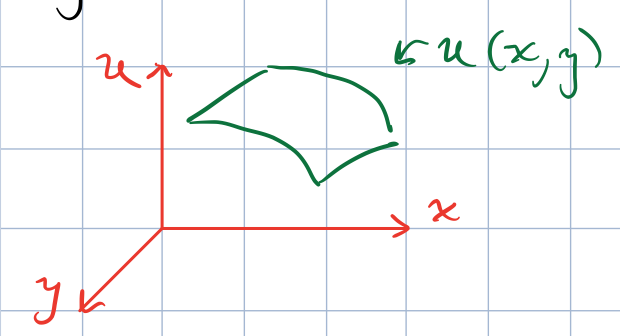
\includegraphics[scale=.75]{fig/fig1_method_characteristics.png}
	\caption{\captionStroke{Schematic integral surface.}}
	\label{fig_integral_surface}
\end{figure}

A surface $u = u(x, y)$ that solves a Cauchy problem is known as an integral
surface since integration is used to solve these problems. We can write down the
equation of this integral surface as
\begin{equation}
  F(x, y, u) \equiv u(x, y) - u = 0.
\end{equation}
Note that the first $u(x, y)$ is a function, while the second $u$ is a
variable. So for example if
\begin{equation}
  u(x, y) = x - y^2,
\end{equation}
then
\begin{equation}
  F(x, y, u) = x - y^2 - u.
\end{equation}

From vector calculus we know that any vector $\mathbf{n}$ normal to the surface $F = 0$ is given by the gradient
\begin{equation}
  \mathbf{n} = \nabla F =
  \frac{\partial u}{\partial x} \mathbf{i}
  + \frac{\partial u}{\partial y} \mathbf{j}
  - \mathbf{k}.
\end{equation}

\fref[fig_normal_vector] shows a schematic representation of this vector. The
vector is represented pointing downwards since $F = u(x, y) - u$.

\begin{figure}[h!]
	\centering 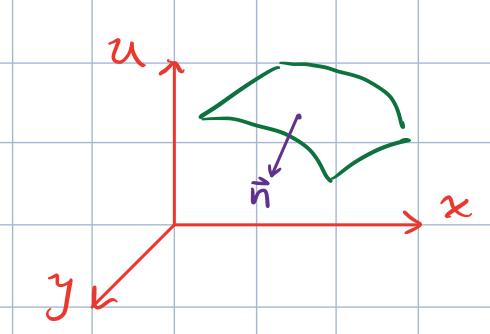
\includegraphics[scale=.75]{fig/fig2_method_characteristics.png}
	\caption{\captionStroke{Schematic integral surface with normal vector.}}
	\label{fig_normal_vector}
\end{figure}

We can rewrite the PDE as a dot product of the form
\begin{equation}
  \left\langle a(x, y), b(x, y), f(x, y, u) \right\rangle \cdot \mathbf{n} = 0.
\end{equation}

This implies that since the dot product is zero, the vector $\left\langle a(x,
y), b(x, y), f(x, y, u) \right\rangle$ must be normal to $\mathbf{n}$. Since we
stated that the vector $\mathbf{n}$ is normal to the surface $F(x, y, u) = 0$,
any vector $\mathbf{v}$ normal to $\mathbf{n}$ must lie in the tangential plane
to $F = 0$ at every point as depicted in \fref[fig_tangential_vector]
\begin{figure}[h!]
	\centering 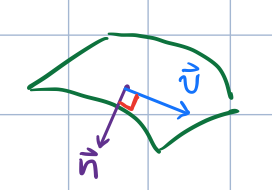
\includegraphics[scale=.75]{fig/fig3_method_characteristics.png}
	\caption{\captionStroke{Schematic integral surface with normal vector
  $\mathbf{n}$ and tangential vector $\mathbf{v}$.}}
	\label{fig_tangential_vector}
\end{figure}

But what do all these details mean? This means that the PDE requires for any
integral surface that solves the equation to be tangential to the vector
\begin{equation}
  \mathbf{v} = a(x,y) \mathbf{i} +
  b(x, y) \mathbf{j} +
  f(x, y, u) \mathbf{k}.
\end{equation}
That is, if we start at some point set by the initial condition and we move in
the direction of the vector $\mathbf{v}$ (which we can determine just by looking
at the PDE) then we move along a curve that lies entirely within the surface
$F = 0$. This curve, depicted in \fref[fig_characteristic_curve] is called a
\textit{characteristic curve}. And by finding the collection of these
characteristic curves we can therefore reconstruct the entire integral surface,
solving therefore the PDE.
\begin{figure}[h!]
	\centering \includegraphics[scale=.75]{fig/fig4_method_characteristics.png}
	\caption{\captionStroke{Schematic of a characteristic curve on an integral
  surface.}}
	\label{fig_characteristic_curve}
\end{figure}

In other words, so far we have shown that given an initial condition
$u(x, 0) = u_0(x)$ as long as we move along the direction given by the vector
$\mathbf{v} = \left\langle a(x,y), b(x,y), f(x,y,u) \right\rangle$ we are
guaranteed to lay on the integral surface. So the process to reconstruct the
entire surface would be to choose a value for $x$, then start at $u_0(x)$ and
move along $\mathbf{v}$; then we would choose a new value of $x$ and repeat the
process. At the end, the union of all these paths along the integral surface
will determine entirely the solution of the PDE. The advantage of the method as
we will show is that walking along the characteristic curve is equivalent to
solving an ODE, which for many cases we know how to do.

We can describe all the points on a characteristic curve by parametrizing
the curve with a vector function
\begin{equation}
  \mathbf{p}(t) = x(t) \mathbf{i} + y(t) \mathbf{j} + u(t) \mathbf{k}.
\end{equation}
Furthermore, we can obtain a vector tangential to this curve $\mathbf{p}(t)$ by
differentiating with respect to the parametrization variable $t$, i.e.
\begin{equation}
  \mathbf{p}'(t) = x'(t) \mathbf{i}+ y'(t) \mathbf{j} + u'(t) \mathbf{k}.
\end{equation}

Since the curve $\mathbf{p}(t)$ lays on the integral surface $F = 0$, and
$\mathbf{p}'(t)$ is tangential to this curve, that means that $\mathbf{p}'(t)$
also lies on the surface.

We stated earlier that if we move along the direction of $\mathbf{v}$ we will
reconstruct the path of the characteristic curve which we now parametrized as
$\mathbf{p}(t)$. That implies that $\mathbf{v}$ and $\mathbf{p}'(t)$ must be
pointing in the same direction, i.e.
\begin{equation}
  \mathbf{p}'(t) = \lambda \mathbf{v},
\end{equation}
where $lambda$ is a scalar. This can also be written as
\begin{equation}
  x'(t)\mathbf{i} + y'(t)\mathbf{j} + u'(t)\mathbf{k} =
  \lambda a(x,y) + \lambda b(x,y) + \lambda f(x,y,u).
\end{equation}
in other words
\begin{align}
  x'(t) = \lambda a(x,y),\\
  y'(t) = \lambda b(x,y), \\
  u'(t) = \lambda f(x,y,u).
\end{align}
We can now solve for $\lambda$ and equate all of the solutions, obtaining
\begin{equation}
  {{dx \over dt} \over a(x,y)}} =
  {{dy \over dt} \over b(x,y)} =
  {{du \over dt} \over f(x,y,u)},
\end{equation}
or simply in a compact differential form
\begin{equation}
  {dx \over a} = {dy \over b} = {du \over f}.
\end{equation}

	%	\pagebreak
\phantom{This ensures that the next section starts on a new page}
\pagebreak
\section{To Do}

\begin{itemize}	
%	\item Get distribution of error from Jane's paper. 
%	\begin{itemize}
%		\item Use Jane's closed form solution and write this up in our paper
%		
%		\item Also consider doing (numerically, not analytically) a 3-state context
%		with an empty promoter. See if the numerical result is any different from
%		Jane's 2-state solution.
%		
%		\item Read Peter Swain's paper "Analytical distributions for stochastic gene
%		expression" to see how to get from Jane's mRNA profile to the gene expression
%		profile. Manuel thinks that we lose some information at every step of the
%		central dogma (see "Data processing inequality" in my Chrome Bookmarks) and
%		that if we can get the gene expression prediction/experiment to match then we
%		can try to measure the mRNA levels directly and see if they also match the
%		prediction. That would be a really nice match between theory and experiment.
%		Manuel and I should discuss the derivations in Peter Swain's paper go.
%	\end{itemize}
	
	\item As per Swain's last point before the Discussion, if the RNAP and repressor's binding-unbinding rates are fast, then the 3-stage model reduces to the 2-stage model with $a \to \frac{\kappa_0}{\kappa_0 + \kappa_1} a$, where $\frac{\kappa_0}{\kappa_0 + \kappa_1}$ is the fraction of the time that the system is in the RNAP bound state in equilibrium.
	\begin{itemize}
		\item Figure out experimentally what these rate constants are for our system
		
		\item Rob has previously suggested that Jeff Gelles knows what many of these rate constants are for the Lac system
		
		\item If these rate constants are fast, we can use the much simpler 2-stage model protein distribution, and we can also easily add in the empty promoter stage (i.e. a 4-stage model) if we just modify $a$ accordingly
	\end{itemize}
	
	\item Expand Swain's 3-stage model (promoter either RNAP bound or repressor bound) to a 4-stage model. I think this should be straightforward to do analytically.
	
	\item Explore the channel capacity analytically in the limit of small noise (discuss whether this is a valid assumption from our data). \textbf{As a starting point, look at Rieckh and Tkacik's ``Noise and information transmission in promoters with multiple internal states''}
	
	\item Other things that would be very interesting to explore:
		\begin{itemize}
			\item Be theorists, and consider how other variables affect the channel capacity. For example, the (active) repressor-DNA binding energy, or $K_A/K_I$, or the rates in the problem. Would be really cool to basically look at the effects of all of the variables that we have on channel capacity, and consider which yield the coolest results.
			\item Varying cross all $R$ and $k_{off}$ values, what is the maximal channel capacity you can achieve?
			\item Potentially look at Mitch Lewis's strains which will have different $K_{DNA}$ or $K_{A}$ and $K_{I}$ parameters and redo the analysis there, showing that the theory is amazingly good!
		\end{itemize}
	
	
	\item \textcolor{blue}{Really important reference for us is \cite{Hansen2015}.
		\begin{itemize}
			\item (Page 6, Figure 2A) Their measured channel capacity for amplitude modulated (AM) signal, was 1.3 for the natural promoter. We are also planning to measure this AM signal, but not the frequency modulated (FM) signal that they also measured.
			\item (Page 7) "Measuring mutual information in a cell population subject to extrinsic noise...underestimates the intrinsic information transduction capacity of a promoter." They claimed this was caused by cells being at different stages of the cell cycle. After correcting for this error, they measured a channel capacity of 1.5, which still means the system can only distinguish between two or three input states
			\item (Page 8) They made a mutant promoter that had a channel capacity of ~2. I assume we are not going to pursue this angle, but it shows that natural operators do not necessarily maximize channel capacity.
			\item Overall, I found it difficult to understand what change in channel capacity was "significant." They claimed that an increase of 0.15 is "small but robust," but I wondered whether this was comparable to their experimental noise. I am worried that if the Lac system also yields small channel capacities, we will end up making statements like "we saw a 0.1 increase in channel capacity between O2 and O1..."
			\item To rephrase that last point, we hope that the Lac system can distinguish multiple inputs (what they call the Rheostat Model), but if channel capacity is ~1 then you can only distinguish the OFF and ON state (i.e. their Noisy Switch Model). Based on your calculations of channel capacity so far, how many bits do you suspect we will find?
			\item I think our paper needs to go \textit{beyond} this paper in a meaningful way. One way I think we will improve upon their results is that we have a \textbf{theoretical prediction} for the form of the variability in gene expression. We should really stress that!
		\end{itemize}
	}
	
	\item \textcolor{blue}{Another important reference \cite{Chevalier2015}:
		\begin{itemize}
			\item Several other groups are making similar mutual information measurements (between ligand concentration and gene expression) in their systems, and so we should really stress what is new about our paper - that we are \textit{predicting everything theoretically}! References 6-10 from this paper should be good to cite.
			\item I really like their short and sweet introduction on mutual information: ``Mutual information (MI) is a natural metric for characterizing information transmission between the inputs of a stochastic network and its nodes. MI quantifies the level of precision with which a given node(s) in a network estimates and responds to an input(s) by accounting for both the mean and variability in the response.''
			\item They also claimed that our theoretical measurements should overestimate the measured mutual information because of: (1) variability of cell's being at different stages of the cell cycle and (2) variability that is extrinsic to the pathway. We can keep that in mind if we theoretically overshoot the measured values.
			\item Finally, they point out that the measured mutual information is time-dependent, so we need to be super careful about making all of our measurements using precisely the same method. Hopefully the O1, O2, O3, Oid strains all grow at exactly the same speed, because otherwise if you always wait until OD 0.5 (or whatever) but this waiting time is different between strains, that could introduce a bias into the measurements.
		\end{itemize}
	}
	
%	\textcolor{brown}{
%	\item (Paper 2) How can the theory be applied to an evolutionary context? For example, compete RBS 1027 against RBS 446, and predict both which will win and exactly by how much. Then unconstrain the system and let them evolve over time on the growth rate versus mutual information graph and see that they (hopefully) move upwards. (May need to make new strains that have LacI and possibly SacB for this)
%	\begin{itemize}
%		\item Cost/benefit function. Do we use Lassig Paper (Nonlinear fitness landscape of a molecular pathway), Uri Alon paper, or our own? (At the very least, should try both cost/benefit functions and see if they give different results.)
%		\item Make a strain as close to optimal as possible. Manuel tried doing this, but got unphysical parameters. Wiggle, wiggle, wiggle them until they are reasonable. Noah is willing to help on this end, if desired (potentially as another member of the project, if desired).
%		\item We agree that there is evolutionary pressure to move up in the growth rate plot, but is there any pressure to move left or right (other than being able to access more upwards space the further you go to the right). Give readers some intuition on what it means for two points to be on the same horizontal line (i.e. what could their profiles look like); what about two vertical points? Do these points have smaller errors, or must they have different curve shapes? Can we make a phase diagram in some way of the different Mutual Info/Growth Rate plot? If you take any curve and scale its error bars up or down, what trajectory do you get on the Mutual Info/Growth Rate plot?
%		\item Keep in mind that we are trying to maximize \textit{growth rate} and not \textit{mutual information}. To be honest about this, we should talk a bit about a strain that maximizes mutual information at the cost of growth rate. Could there be some other metric that is analogous to growth rate and still uses the full distribution?
%	\end{itemize}
%	\item (Future) Does the natural Lac operon provide qualitatively different behavior than the synthetic ones? Explore this theoretically, and if it does then we could potentially make these strains as well.
%	}
\end{itemize}
	% Bibliography
	\bibliographystyle{unsrt}
	\bibliography{./chann_cap_bib}
\end{document}
